\documentclass[11pt,a4paper]{article}

\usepackage[utf8]{inputenc}
\usepackage[T1]{fontenc}
\usepackage[margin=2.5cm]{geometry}
\usepackage{amsmath,amssymb,amsthm,mathtools}
\usepackage{xcolor}
\usepackage{microtype}
\usepackage{enumitem}
\usepackage{tcolorbox}
\usepackage{tikz}
\usetikzlibrary{arrows.meta}
\usepackage{booktabs,array}
\usepackage{fancyhdr}
\usepackage{titlesec}
\usepackage[colorlinks=true,linkcolor=blue!60!black,urlcolor=blue!70!black,citecolor=green!50!black]{hyperref}
\usepackage[capitalize,nameinlink]{cleveref}
% -- Page style and sectional layout --
\definecolor{lectureblue}{RGB}{28,74,120}
\definecolor{lecturegray}{RGB}{65,65,65}
\definecolor{lecturerule}{RGB}{190,205,220}

\pagestyle{fancy}
\fancyhf{}
\setlength{\headheight}{14pt}
\fancyhead[L]{\small\sffamily\color{lecturegray}Toric methods for Calabi--Yau compactifications}
\fancyhead[R]{\small\sffamily\color{lecturegray}ESI 2026}
\fancyfoot[C]{\small\sffamily\color{lecturegray}\thepage}
\renewcommand{\headrulewidth}{0.4pt}
\renewcommand{\footrulewidth}{0pt}
\fancypagestyle{plain}{%
  \fancyhf{}%
  \fancyfoot[C]{\small\sffamily\color{lecturegray}\thepage}%
  \renewcommand{\headrulewidth}{0pt}%
}

\titleformat{\section}
  {\Large\sffamily\bfseries\color{lectureblue}\raggedright\sloppy}
  {\thesection}{0.75em}{}
  [\vspace{0.35ex}{\color{lecturerule}\titlerule[0.7pt]}]
\titleformat{name=\section,numberless}
  {\Large\sffamily\bfseries\color{lectureblue}\raggedright\sloppy}
  {}{0pt}{}
  [\vspace{0.35ex}{\color{lecturerule}\titlerule[0.7pt]}]
\titleformat{\subsection}
  {\large\sffamily\bfseries\color{lectureblue}\raggedright}
  {\thesubsection}{0.75em}{}
\titleformat{\subsubsection}
  {\normalsize\sffamily\bfseries\color{lectureblue}\raggedright}
  {\thesubsubsection}{0.75em}{}
\titlespacing*{\section}{0pt}{3.0ex plus 1ex minus .2ex}{1.8ex plus .2ex}
\titlespacing*{\subsection}{0pt}{2.3ex plus .8ex minus .2ex}{1.0ex plus .2ex}
\titlespacing*{\subsubsection}{0pt}{1.8ex plus .6ex minus .2ex}{0.8ex plus .2ex}

% -- Math conventions used throughout --
\newcommand{\KC}{\mathcal{K}}
\newcommand{\eKC}{\widetilde{\mathcal{K}}}
\newcommand{\MC}{\mathcal{M}}
\newcommand{\Pl}{M_{\mathrm{Pl}}}
\newcommand{\Nef}{\mathrm{Nef}}
\newcommand{\Vol}{\mathcal{V}}
\newcommand{\Hol}{\mathrm{Hol}}
% -- Macros used by the appendix --
\newcommand{\Pic}{\mathrm{Pic}}
\newcommand{\Cl}{\mathrm{Cl}}
\newcommand{\as}[1]{{\color{red}AS: #1}}
\newcommand{\revision}[1]{{\color{blue!70!black}#1}}

% Public build controls.  Lecture 4 is a separate talk by default.
% The appendices remain compiled as reference material because the main
% lectures cite labelled statements from them.
\newif\ifincludelecturefour
\includelecturefourfalse
\newif\ifincludeappendices
\includeappendicestrue

% -- Theorem environments (used; see TASI register) --
\theoremstyle{plain}
\newtheorem{definition}{Definition}[section]
\newtheorem{theorem}[definition]{Theorem}
\newtheorem{proposition}[definition]{Proposition}
\newtheorem{lemma}[definition]{Lemma}
\newtheorem{corollary}[definition]{Corollary}
\theoremstyle{definition}
\newtheorem{example}[definition]{Example}
\theoremstyle{remark}
\newtheorem{remark}[definition]{Remark}
\theoremstyle{definition}
\newtheorem{exercise}[definition]{Exercise}
\numberwithin{equation}{section}


\title{\textbf{Toric methods for Calabi--Yau compactifications\\
and the string landscape}\\[0.8em]
\large Lecture notes for ESI 2026 programme on \\[0.4em]
 \emph{The Unreasonable Effectiveness of Toric Geometry:}\\
 \emph{Bridging Mathematics, Computation, and String Theory}\\
}
\date{Lectures: 22--24 June 2026}
\author{\large\textbf{Andreas Schachner}}


\begin{document}
\maketitle
\thispagestyle{empty}


\tableofcontents

%!TEX root = ../main.tex

% ==================================================================
\section*{Scope and lecture outline}
\phantomsection
\addcontentsline{toc}{section}{Scope and lecture outline}

These lectures are an introduction to \textbf{toric methods for
Calabi--Yau compactifications and the string landscape} for
mathematicians.  The organising
question is concrete: how much of a four-dimensional effective theory,
and in particular of its vacuum energy, can be computed from explicit
algebraic and toric data?  The candidate de~Sitter construction of
\cite{McAllister:2024lnt} is the central worked example, but the first
goal is more basic: to explain why explicit Calabi--Yau geometry is
needed at all.

The basic toric vocabulary (fans, cones, divisors, the secondary
fan etc.) is used throughout without being re-derived in the live
lectures; it is collected in the appendices. By contrast, the
constructions that are central to the worked example, in particular
Batyrev's construction of Calabi--Yau hypersurfaces from reflexive
polytopes and the role of FRSTs, are re-derived at the level of a
stated theorem in Lecture~1 (see Theorem~\ref{thm:batyrev}). The
appendices collect the definitions and standard results from algebraic
geometry, convex geometry, toric geometry, mirror symmetry,
orientifolds, and computational workflows that are needed to read the
notes as a self-contained reference.

Sections marked by an asterisk are included for completeness and for
later reference, but they are not part of the intended blackboard
delivery. In the live lectures I will use them only as optional
background or as answers to questions.

\medskip
\noindent\textbf{Prerequisites.}
\begin{itemize}[nosep,leftmargin=*]
    \item Algebraic and complex geometry at the level of Huybrechts
    (\emph{Complex Geometry} \cite{Huybrechts:2005complex}) or
    Voisin (\emph{Hodge Theory and Complex Algebraic Geometry}
    \cite{Voisin:2002}).
    \item Toric geometry at the level of Cox--Little--Schenck
    \cite{cox-little-schenck:toric}: fans, divisors, intersection
    rings, the K\"ahler and Mori cones, the secondary fan, and
    reflexive polytopes. Batyrev's construction
    \cite{Batyrev:1993oya} and the Kreuzer--Skarke list
    \cite{Kreuzer:2000xy} are helpful background but are recalled in
    Lecture~1 (see \Cref{ssec:L1-toric}).
    \item Riemannian and Hermitian geometry: holonomy and the Hodge
    decomposition. Berger's classification is helpful background but
    is restated in Lecture~1 (see \Cref{thm:berger}).
    \item Basic physics vocabulary is helpful but not assumed: fields,
    actions, equations of motion, compactification, fluxes, branes,
    and effective field theory are introduced when first used.
\end{itemize}


\medskip
\noindent\textbf{Motivation.}
The motivation is two-fold. First, the notes explain how toric
geometry makes certain string compactifications explicit enough that
one can compute physical quantities rather than only discuss them
abstractly. The conceptual ingredients have long been established:
Calabi--Yau geometry, mirror symmetry, Picard--Fuchs equations,
Gopakumar--Vafa invariants, D-branes, and four-dimensional
supergravity have all been studied for decades. What has changed is
the feasible computational range. Many calculations that were once
limited to one- or few-modulus examples can now be attempted for the largest known Hodge numbers, i.e., compactifications with hundreds of moduli, provided one keeps careful control of
truncations and chamber structure.

Second, the notes are meant to identify bottlenecks. 
The concrete questions are geometric before they are
physical. Given a Calabi--Yau threefold $X$, how does one determine
its K\"ahler cone, effective cone etc.?
How does one compute minimal-volume representatives of divisor
classes, especially when holomorphic representatives exist only after
moving in the space of birational equivalence classes of $X$? Which effective divisors have
$h^\bullet(D,\mathcal{O}_D)=(1,0,0)$ and can therefore contribute to
the non-perturbative superpotential? How should one compare the Wall
data of hypersurfaces arising from different triangulations, and how
many inequivalent geometries are really present in the
Kreuzer--Skarke ensemble? 
The hope is that the lectures make these questions precise enough to
be useful to both the mathematics and string theory communities.

\medskip
\noindent\textbf{Lecture outline.}
The live blackboard narrative is deliberately narrower than the
written notes: compactification first selects Ricci-flat internal
geometries; the deformations of those geometries become
four-dimensional moduli; fluxes, sources and quantum corrections
generate a scalar potential $V$; and toric geometry supplies much
of the discrete data needed to write and analyse that potential. The
detailed explanation of how ten-dimensional fields reduce to
four-dimensional fields appears only after the Calabi--Yau moduli
have been introduced. In this sense the purpose is not to give a
general survey of string theory, but to explain why explicit
geometry is needed to compute its four-dimensional consequences.



There is intentional overlap with the TASI lectures
\cite{McAllister:2025qwq}. The TASI notes are the physics-first
reference for the Type IIB flux compactification, the leading-order
effective field theory, and the candidate de~Sitter construction.
The present notes reorganise that material for the ESI audience: the
blackboard route starts from compact Ricci-flat geometry, then
explains which toric computations supply the input to the
four-dimensional scalar potential. Whenever a statement is imported
from the TASI treatment rather than rederived here, the relevant TASI
section is cited explicitly.

\begin{enumerate}[leftmargin=*]
    \item \textbf{Lecture~1: The why and how of Calabi--Yau.}
    The first lecture introduces the minimal string theory input,
    explains why compactification leads to a
    Ricci-flat internal geometry, why Calabi--Yau threefolds are the
    computable and best understood class used in these notes, and how
    Batyrev's construction turns reflexive polytopes and FRSTs into
    explicit Calabi--Yau hypersurfaces in toric varieties. The emphasis
    is pragmatic: what toric methods compute reliably today
    (Hodge data, intersection numbers, cones, divisor topology), and
    what remains beyond current algorithms.
    Along the way we preview where these data enter physics: flux
    superpotentials, instanton corrections, divisor zero-mode tests,
    and K\"ahler-cone navigation.

    \item \textbf{Lecture~2: Periods and GV invariants from toric data.}
    The second lecture introduces the minimal Type IIB/O3--O7
    dictionary needed to write the flux superpotential and then
    focuses on the main computational problem:
    \begin{equation}
        W_{\rm flux}=\int_X\Omega\wedge G_3 .
    \end{equation}
    Fluxes supply the integral coefficients; periods supply the
    functions. The lecture explains how mirror symmetry, toric
    hypersurfaces, the mirror map, and genus-zero GV invariants make
    these periods computable. It then uses PFVs as the final
    application: special integral fluxes make the polynomial LCS
    contribution flat, while the GV-controlled instanton terms lift
    the remaining direction and produce a computable small value of
    $W_0$. Non-perturbative K\"ahler-modulus stabilisation and the
    candidate-dS pipeline are deferred to Lecture~3.

    \item \textbf{Lecture~3: Vacuum energies from toric geometry.}
    The third lecture assembles the leading-order effective
    theory for Type IIB O3/O7 orientifold compactifications with flux,
    non-perturbative K\"ahler-modulus stabilisation, and a
    redshifted antibrane uplift. It introduces
    geometric phases, flop transitions, vex chambers, and the
    extended K\"ahler cone,
    then explains how chamber-aware algorithms, including
    \texttt{fanroots} and \texttt{JAXVacua}, locate
    K\"ahler moduli critical points. The remaining ingredients are the
    Klebanov--Strassler throat, KPV anti-D3 uplift, the explicit
    toric AdS precursor and candidate-dS recipes, and the control
    checks: tadpoles, GV convergence, higher-order corrections,
    backreaction, and quantisation issues. The list is retained
    because these checks distinguish the leading-order candidate
    construction from a fully controlled vacuum theorem.
\end{enumerate}

% ==================================================================
\setcounter{section}{0}


%!TEX root = ../main.tex

% ==================================================================
\section{Lecture~1: The why and how of Calabi--Yau}\label{sec:L1}

\medskip

\noindent\textit{Anchor:} TASI \cite{McAllister:2025qwq},
\S\S\,1--2.

\medskip
\noindent\textit{Guiding question.} What can toric methods compute
for string compactifications, and where do current methods still
fall short?

The answer will be deliberately two-sided. Toric geometry gives an
explicit, computable supply of Calabi--Yau threefold hypersurfaces:
Hodge numbers, intersection forms, cones, divisor topology, periods,
and enumerative inputs such as Gopakumar--Vafa invariants can be
extracted algorithmically. It does not, by itself, solve the
Ricci-flat metric, determine every effective curve or divisor on the
hypersurface, or provide access to all quantum corrections.

\medskip
\noindent\textit{Historical and computational thread.}
The geometric problem starts with two classical inputs. Yau's
solution of the Calabi conjecture implies the existence of
Ricci-flat K\"ahler metrics on compact K\"ahler manifolds with
trivial canonical bundle \cite{Yau:1978cfy}, while Calabi--Yau
threefolds entered string compactification through the work of
Candelas, Horowitz, Strominger and Witten
\cite{Candelas:1985en}. The reason these lectures focus on toric
hypersurfaces is more computational: Batyrev's reflexive polytopes
give a large, explicit class of mirror pairs
\cite{Batyrev:1993oya}; the Kreuzer--Skarke classification makes
this class finite and searchable \cite{Kreuzer:2000xy}; and modern
packages such as \texttt{CYTools} turn the resulting combinatorial
data into the intersection, cone and divisor-topology inputs used
later \cite{Demirtas:2022hqf}. Lecture~1 explains enough of this
chain to make Lectures~2 and~3 self-contained.

\medskip
\noindent\textit{Goals.} After this lecture you can
\begin{enumerate}[nosep,leftmargin=*]
    \item state what a string compactification is, as a geometric
    object, and why the vacuum Einstein equations on a product ansatz
    select Ricci-flat internal manifolds;
    \item explain why Calabi--Yau threefolds are the computable
    Ricci-flat class used in these lectures, and how reduced holonomy
    gives the parallel spinors responsible for residual
    supersymmetry;
    \item identify the moduli of a Calabi--Yau compactification with
    specific cohomological data;
    \item explain why Calabi--Yau hypersurfaces in toric varieties
    are the natural constructive source of explicit compact examples,
    and what data they feed into Lectures~2 and~3.
\end{enumerate}


\subsection{Why string theory, and why compactify?}



Let us motivate how geometry enters physics.
We have very successful but structurally different theories
for matter and gravity:
\begin{equation}
\begin{array}{lll}
\text{matter} &:&
  \begin{array}[t]{l}
    \text{Standard Model},\\
    \text{\emph{language:} quantum field theory},\\
    \text{\emph{hypothesis:} point particles};
  \end{array}
\\[1.2em]
\text{gravity} &:&
  \begin{array}[t]{l}
    \text{General Relativity},\\
    \text{\emph{language:} differential geometry},\\
    \text{\emph{hypothesis:} spacetime as a manifold}.
  \end{array}
\end{array}
\end{equation}
The quantum gravity problem is to find a framework in which these two
descriptions can be combined.  Perturbative quantum gravity based on
point particles is not perturbatively renormalisable, and curvature
singularities indicate that the classical spacetime description
itself can break down.  String theory is one proposed framework in
which the fundamental extended objects are one-dimensional strings
rather than point particles.

\begin{figure}
\begin{center}
\centering
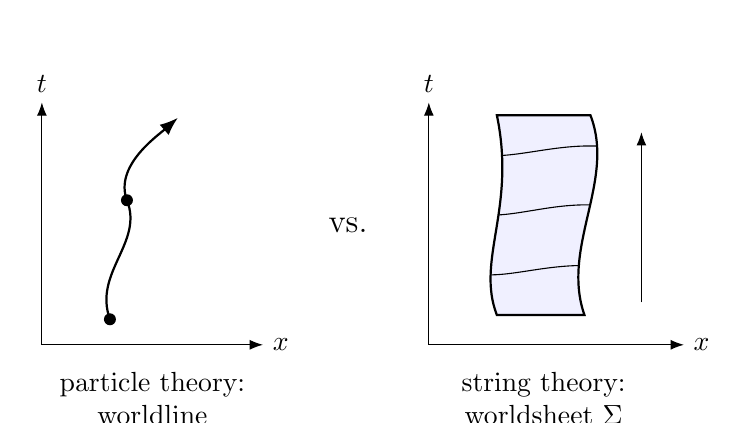
\begin{tikzpicture}[scale=1.08,>=Latex]
  \begin{scope}
    \draw[->,thin] (-0.25,-0.15) -- (2.35,-0.15) node[right] {$x$};
    \draw[->,thin] (-0.25,-0.15) -- (-0.25,2.70) node[above] {$t$};
    \draw[thick,->] (0.55,0.15)
      .. controls (0.35,0.70) and (0.95,1.05) .. (0.75,1.55)
      .. controls (0.60,1.95) and (1.10,2.30) .. (1.35,2.52);
    \fill (0.55,0.15) circle (2pt);
    \fill (0.75,1.55) circle (2pt);
    \node[align=center] at (1.05,-0.78) {particle theory:\\ worldline};
  \end{scope}

  \node at (3.35,1.25) {\large vs.};

  \begin{scope}[xshift=4.55cm]
    \draw[->,thin] (-0.25,-0.15) -- (2.75,-0.15) node[right] {$x$};
    \draw[->,thin] (-0.25,-0.15) -- (-0.25,2.70) node[above] {$t$};
    \path[fill=blue!6]
      (0.55,0.20)
      .. controls (0.30,0.85) and (0.78,1.45) .. (0.55,2.55)
      -- (1.65,2.55)
      .. controls (1.95,1.78) and (1.30,1.00) .. (1.58,0.20)
      -- cycle;
    \begin{scope}
      \clip
        (0.55,0.20)
        .. controls (0.30,0.85) and (0.78,1.45) .. (0.55,2.55)
        -- (1.65,2.55)
        .. controls (1.95,1.78) and (1.30,1.00) .. (1.58,0.20)
        -- cycle;
      \draw[thin] (0.15,0.72)
        .. controls (0.65,0.55) and (1.18,0.90) .. (2.05,0.74);
      \draw[thin] (0.15,1.42)
        .. controls (0.70,1.25) and (1.24,1.62) .. (2.05,1.45);
      \draw[thin] (0.15,2.12)
        .. controls (0.70,1.95) and (1.28,2.30) .. (2.05,2.15);
    \end{scope}
    \path[draw,thick]
      (0.55,0.20)
      .. controls (0.30,0.85) and (0.78,1.45) .. (0.55,2.55)
      -- (1.65,2.55)
      .. controls (1.95,1.78) and (1.30,1.00) .. (1.58,0.20)
      -- cycle;
    \draw[->,thin] (2.25,0.35) -- (2.25,2.35);
    \node[align=center] at (1.10,-0.78) {string theory:\\ worldsheet $\Sigma$};
  \end{scope}
\end{tikzpicture}
\end{center}
\vspace*{-0.5cm}
\caption{A point particle sweeps out a
one-dimensional worldline, whereas a string sweeps out a
two-dimensional worldsheet.  In both panels the object evolves upward
in target time $t$: the point traces a curve, while the spatially
extended string traces a strip. }
\end{figure}

The useful contrast is the following. A particle
traces out a worldline in spacetime; a string traces out a worldsheet
$\Sigma$, and the simplest classical action is proportional to its
area,
\begin{equation}
    S_{\rm NG}=-T\int_{\Sigma}\mathrm{d}A \, ,
\end{equation}
where $T$ is the string tension. Quantising the string gives a
tower of vibrational modes. 
In the point-particle picture
one quantises the possible motions of a point; in the string picture
one also quantises the normal modes of an extended object.  Very
schematically,
\begin{equation}
    \text{particle: worldline}
    \qquad\longrightarrow\qquad
    \text{string: worldsheet with oscillator modes}\, .
\end{equation}
The word ``harmonics'' here refers to these oscillator modes of the
string.  After quantisation they appear, from the spacetime point of
view and for an observer sufficiently far away, as different particle
species: scalars, gauge fields, spinors, and a spin-$2$ graviton
among them.


It is useful to separate two attitudes.  One can use
string theory and related constructions as mathematical
tools in broader effective descriptions.  In these lectures we use
the stronger quantum gravity interpretation: the theory is required
to include gravity, and the perturbative spectrum contains a
spin-$2$ graviton.  With this interpretation, the consistency
conditions of the quantum theory are part of the input.  In
particular, for the critical superstring the consistency of the quantum theory fixes the target spacetime dimension to ten.
At energies small compared with the
string scale, one keeps only the massless modes. 
The massive oscillator modes have masses of order the string
scale $M_s$, so a low-energy observer with characteristic energy
$E\ll M_s$ cannot excite them as dynamical fields.  Their effects are
still present indirectly, through higher-derivative corrections to
the effective action.
The one fact from
this construction that Lecture~1 needs is that the massless spectrum
of a consistent superstring includes a ten-dimensional metric,
together with further geometric fields such as differential forms,
scalars, spinors, and gauge fields. The metric is what will make
Ricci-flat geometry enter immediately.

Since observed physics is effectively
four-dimensional at accessible energies, a compactification must
explain how a ten-dimensional theory can give a four-dimensional
effective theory:
\begin{equation}
    \dim \mathcal{M}_{10}=10=9+1,
    \qquad
    \dim \mathcal{M}_4=4=3+1,
    \qquad
    \mathcal{M}_{10}\simeq \mathcal{M}_4\times X .
\end{equation}
The compact six-dimensional factor $X$ is where geometry enters.
The central point of the lectures is that the topology and geometry
of $X$ determine the light four-dimensional fields, their
couplings, and the scalar potential whose critical values are the
vacuum energies.




\subsection{Framing: what a string compactification is}\label{ssec:L1-framing}

For the first lecture, the input from string theory can be stated
without choosing a specific string theory. It is the following
geometric package.

\begin{enumerate}[leftmargin=*]
    \item A \emph{ten-dimensional spacetime} $\mathcal{M}_{10}$:
    a Lorentzian $10$-manifold with metric $g_{MN}$.
    \item Additional \emph{fields} $\Phi$ on $\mathcal{M}_{10}$.
    Here a field simply means a geometric object varying over
    spacetime: a section of a vector bundle, such as a differential
    form, a function, a connection, a spinor, or the metric itself.
    In Lecture~1 we keep these fields mostly silent and set them to zero or
    to constants when deriving the Ricci-flatness condition.
    \item \emph{Source terms and charged objects}, such as branes
    and orientifold planes,
    which enter through $\mathcal{L}_{\rm source}$ and produce
    localised stress-energy and charge.
    A brane is an extended object on which open strings can
    end, or more generally an object carrying charge under one of the
    differential-form gauge fields of the theory.  Its worldvolume is
    a submanifold of spacetime, so after compactification a brane can
    wrap a cycle in $X$ and fill some or all of the visible
    four-dimensional spacetime.  This is why branes are simultaneously
    geometric objects and physical sources: they contribute localised
    energy-momentum, carry quantised charge, and can support gauge
    fields or matter in the four-dimensional theory
    \cite{Polchinski:1996na}.
    \item An \emph{action functional}
    \begin{equation}
        S[g,\Phi]
        =
        \frac{1}{2\kappa_{10}^2}\int_{\mathcal{M}_{10}}
        \mathrm{d}^{10}x\,\sqrt{-g}\,
        \bigl(R^{(10)}+\mathcal{L}_{\rm matter}(g,\Phi)
        +\mathcal{L}_{\rm source}(g,\Phi)+\underbrace{\ldots}_{\mathrm{e.g.}\, R^4}\bigr)\, ,
    \end{equation}
    whose Euler--Lagrange equations are the equations of motion,
    i.e., the differential equations obtained by requiring the first
    variation of $S$ to vanish, see Eq.~\eqref{eq:EOMRvac} below.
    This is the classical, leading-order ten-dimensional action.
    The full string effective action also contains
    higher-derivative and quantum corrections.\footnote{The first well-known perturbative
    correction to the ten-dimensional type-II action contains an
    $R^4$ term at order $(\alpha')^3$. The
    parameter $\alpha'$ is the inverse string tension, up to the
    conventional factor $2\pi$, and sets the square of the string
    length.  Corrections in powers of $\alpha'$ are higher-derivative
    or finite-string-size corrections.  The string coupling $g_s$
    controls the loop expansion.}
    We do not include those corrections in the first-pass
    vacuum equation, but they reappear in Lecture~2 as corrections to
    the four-dimensional effective action.
\end{enumerate}

Let $x^\mu$ be coordinates on a four-dimensional Lorentzian manifold
$\mathcal{M}_4$ and $y^m$ coordinates on a compact real
$6$-manifold $X$. A warped product metric on
$\mathcal{M}_{10}=\mathcal{M}_4\times X$ has the form
\begin{equation}\label{eq:L1-warped-ansatz}
    \mathrm{d}s^2_{10}
    =
    \mathrm{e}^{2A(y)}\,g^{(4)}_{\mu\nu}(x)\,\mathrm{d}x^\mu \mathrm{d}x^\nu
    +
    \mathrm{e}^{-2A(y)}\,g^{(6)}_{mn}(y)\,\mathrm{d}y^m \mathrm{d}y^n .
\end{equation}
The function $A(y)$ is the \emph{warp factor}. In the first pass
through the vacuum equations we set $A=0$, so the metric is the
ordinary product metric
$\mathrm{d}s^2_{10}=\mathrm{d}s^2(\mathcal{M}_4)+\mathrm{d}s^2(X)$.
This is the Kaluza--Klein bridge in its simplest form: a
four-dimensional observer does not see the internal coordinates
directly, but sees the coefficients of expansions in functions,
forms, and metric deformations on $X$.

\begin{definition}[String compactification, geometrically]
A \emph{string compactification} consists of:
(i) a factorisation $\mathcal{M}_{10} = \mathcal{M}_4\times X$
of the ten-dimensional spacetime into a four-dimensional Lorentzian
manifold $\mathcal{M}_4$ and a compact $6$-dimensional Riemannian
manifold $X$ (the \emph{internal} space);
(ii) a solution of the ten-dimensional equations of motion on
$\mathcal{M}_{10}$ with metric in the warped product form
\eqref{eq:L1-warped-ansatz};
(iii) background choices for any non-metric fields and charged
objects that are present, subject to the global consistency
conditions of the chosen string theory.
\end{definition}

On a compact internal space, closed differential-form field
strengths can have quantised periods. Abstractly, if $F_p$ is a
closed $p$-form field strength, \emph{flux quantisation} means that its
normalised periods over integral $p$-cycles are integers, so the
background defines an integral cohomology class. The precise
normalisation and even the correct cohomology theory depend on the
string theory and on the charged objects present. Lecture~2
specialises this statement to Type IIB, where the flux
superpotential uses the three-form classes
$[F_3],[H_3]\in H^3(X,\mathbb{Z})$.

At this point the lecture has only defined the geometric problem: choose a compact six-manifold $X$, a metric on $\mathcal{M}_4\times X$, and background fields and sources
so that the ten-dimensional equations of motion are satisfied, and
then determine the four-dimensional fields and interactions obtained
by expanding around that solution.
We now first find the internal geometries that can solve the equations of motion in the compactification background, and then ask which four-dimensional fields and
potentials those geometries produce.

\subsection{The vacuum solution problem}\label{ssec:L1-vacuum}

We begin in the simplest setting: no fluxes, no branes. We ask which
Riemannian metrics on $X$ are compatible with a vacuum solution.

The metric equation comes from varying the schematic action above
with respect to $g^{MN}$. Let
\begin{equation}
    S_{\rm matter+source}
    =
    \frac{1}{2\kappa_{10}^2}
    \int \mathrm{d}^{10}x\,\sqrt{-g}\,
    \bigl(\mathcal{L}_{\rm matter}+\mathcal{L}_{\rm source}\bigr)\, ,
\end{equation}
where $\mathcal{L}_{\rm matter}$ contains the kinetic terms of the
non-metric fields $\Phi$ and $\mathcal{L}_{\rm source}$ contains
localised brane/orientifold terms. Define
\begin{equation}
    T_{MN}
    \coloneqq  
    -\frac{2}{\sqrt{-g}}\,
    \frac{\delta S_{\rm matter+source}}{\delta g^{MN}} .
\end{equation}
Then the ten-dimensional Einstein equation is
\begin{equation}\label{eq:EOMRvac} 
    R^{(10)}_{MN}
    =
    \kappa_{10}^2
    \left(T_{MN}-\frac18 g_{MN}T^K{}_K\right).
\end{equation}
In this first pass we set all additional fields to zero or constant
and include no localised sources, so $T_{MN}=0$. The unwarped product
version of \eqref{eq:L1-warped-ansatz} then gives
\begin{equation}
    R_{\mu\nu}^{(4)} = 0 \,, \qquad R_{mn}^{(6)} = 0 \,.
\end{equation}
The four-dimensional Einstein vacuum equation forces $\mathcal{M}_4$
to be Ricci-flat. For our purposes the physically interesting case
is $\mathcal{M}_4 = \mathbb{R}^{1,3}$ (Minkowski), so
$R_{\mu\nu}^{(4)}=0$ holds trivially. The interesting condition is
the internal one: \emph{$X$ must be Ricci-flat}.

The problem is then: construct compact Ricci-flat Riemannian
$6$-manifolds on which one can compute. This is a hard nonlinear PDE
problem: explicit Ricci-flat metrics on compact non-flat
$6$-manifolds are generally not known in closed form. The useful
insight is that one does not need the metric explicitly in order to
build the compactification. Yau's theorem guarantees the
\emph{existence} of Ricci-flat K\"ahler metrics from
complex-geometric data, and toric geometry gives a large explicit
class of spaces for which the relevant topological data are
computable.

\subsection{Berger's holonomy classification}\label{ssec:L1-berger}

The compactification problem above asks for Ricci-flat internal
manifolds with enough structure to control the low-energy theory.
Holonomy is the efficient invariant for this purpose. It records how
tangent vectors, tensors and spinors transform under parallel
transport, and therefore tells us which parallel geometric objects a
metric can admit. 

\begin{theorem}[Berger, holonomy classification \cite{Joyce:2000,Besse:1987}]\label{thm:berger}
Let $(X,g)$ be a simply-connected, complete Riemannian manifold
whose holonomy representation is irreducible and whose metric is
not locally symmetric. Then the (restricted) holonomy group
$\Hol(X,g)\subseteq\mathrm{SO}(\dim X)$ is one
of groups in Table~\ref{tab:berger}.
The lower bounds $m\geq 2$ remove degenerate or duplicated
low-dimensional cases ($\mathrm{U}(1)=\mathrm{SO}(2)$,
$\mathrm{Sp}(1)=\mathrm{SU}(2)$,
$\mathrm{Sp}(1)\!\cdot\!\mathrm{Sp}(1)=\mathrm{SO}(4)$).
\end{theorem}

\begin{table}[t!]
\begin{center}
\begin{tabular}{llll}
\toprule
Holonomy & Dimension & Ricci-flat? & Geometry relevant here \\
\midrule
$\mathrm{SO}(n)$ & $n$ & no generic implication & no parallel spinor in general \\
$\mathrm{U}(m)$ & $2m$ & not necessarily & K\"ahler \\
$\mathrm{SU}(m)$ & $2m$ & yes & Calabi--Yau (Kähler+Ricci-flat) \\
$\mathrm{Sp}(m)$ & $4m$ & yes & hyperk\"ahler \\
$\mathrm{Sp}(m)\!\cdot\!\mathrm{Sp}(1)$ & $4m$ & no (Einstein) & quaternionic K\"ahler \\
$G_2$ & $7$ & yes & $G_2$ manifolds \\
$\mathrm{Spin}(7)$ & $8$ & yes & $\mathrm{Spin}(7)$ manifolds \\
\bottomrule
\end{tabular}
\end{center}
\caption{Berger's list of irreducible
Riemannian holonomies.}\label{tab:berger} 
\end{table}


Berger's theorem is useful here because it sharply limits the
possible irreducible, non-symmetric Riemannian holonomies. It does
\emph{not} classify all compact Ricci-flat manifolds. Rather, it
explains why, once one asks for a six-dimensional irreducible
Ricci-flat background admitting parallel spinors, the natural
holonomy group is contained in $\mathrm{SU}(3)$. In the terminology
of \cite{McAllister:2025qwq}, the compact Ricci-flat
examples used in string compactification all arise from reduced, or
special, holonomy; the Calabi--Yau case is the six-dimensional
member of this list that is complex, K\"ahler, and computationally
accessible. This is a guide to the known constructive landscape, not
a theorem excluding every possible Ricci-flat six-manifold outside
the classes we discuss. 



For a compact K\"ahler threefold, the algebraic-geometric condition
that implements the $\mathrm{SU}(3)$ holonomy target is the
triviality of the canonical bundle.
Let $\mathcal{O}_X$ denote the structure sheaf of holomorphic
functions on $X$; an isomorphism $K_X\cong\mathcal{O}_X$ means that
the canonical bundle is holomorphically trivial, equivalently that
there is a nowhere-vanishing holomorphic $(3,0)$-form.
Holomorphic triviality of $K_X$ gives $c_1(X)=0$;
Yau's theorem then gives a Ricci-flat K\"ahler metric in each
K\"ahler class; and, after excluding flat or product factors, the
holonomy is the expected subgroup of $\mathrm{SU}(3)$,
\begin{equation}
    K_X \cong \mathcal{O}_X
    \quad\Longrightarrow\quad
    \text{Ricci-flat K\"ahler metric}
    \quad\Longrightarrow\quad
    \Hol(X)\subseteq \mathrm{SU}(3)\, .
\end{equation}
When the holonomy is exactly $\mathrm{SU}(3)$, this is the generic
irreducible Calabi--Yau threefold case. Proper subgroups correspond
to extra structure, such as flat factors or product geometries, and
usually to more supersymmetry than the generic threefold case. This
is the precise sense in which Calabi--Yau threefolds are the
workhorse Ricci-flat backgrounds of the lectures: they are explicit
enough to construct and compute with, and their reduced holonomy has
the spinorial consequence needed by the physics.

\subsection{Aside: Reduced holonomy, parallel spinors, and supersymmetry\texorpdfstring{$^{\ast}$}{*}}
\label{ssec:L1-ricci-flat}

Supersymmetry is not the starting point of the geometric argument; it
is a consequence of the reduced holonomy just described. The physics
reason one cares about it is that residual supersymmetry gives
technical control of the low-energy theory and organises the
four-dimensional fields into multiplets. The mathematical statement
is the existence of parallel sections of the spinor bundle.

\begin{definition}[Parallel (covariantly constant) spinor]
Let $(X,g)$ be a Riemannian spin manifold with spinor bundle $S\to X$
and let $\nabla$ denote the spin connection. A \emph{parallel} (or
\emph{covariantly constant}) \emph{spinor} is a smooth section
$\eta\in\Gamma(S)$ with $\nabla \eta = 0$.
\end{definition}

\begin{remark}[Terminology]
In the physics literature these are often called \emph{Killing
spinors}. In the standard differential-geometry convention,
a \emph{Killing spinor} satisfies
$\nabla_X\eta = \lambda\, X\!\cdot\!\eta$ for a nonzero constant
$\lambda$, and the $\lambda=0$ case is called a \emph{parallel}
spinor and treated separately. For the unwarped Minkowski
compactification considered here the relevant case is $\lambda=0$,
and we use the term \emph{parallel} throughout.
\end{remark}

\begin{proposition}[Physics dictionary; standard supergravity
    Killing-spinor analysis,
    \cite{McAllister:2025qwq} \S\,2.3]\label{thm:susy-parallel}
For the configuration $\mathcal{M}_4 \times X$ with
$\mathcal{M}_4 = \mathbb{R}^{1,3}$, the unwarped product metric,
no fluxes, and no branes, vanishing of the supergravity SUSY
variations on the four-dimensional vacuum requires that $X$ admit
a parallel spinor. Starting from a ten-dimensional Type II theory
with thirty-two real supercharges, one independent complex parallel
spinor on $X$ corresponds to $\mathcal{N}=2$ four-dimensional
supersymmetry (eight real supercharges) before any orientifold
projection; starting instead from a heterotic or Type I theory
(sixteen real supercharges in ten dimensions), the same condition
yields $\mathcal{N}=1$ in four dimensions (four real supercharges),
as in Candelas--Horowitz--Strominger--Witten
\cite{Candelas:1985en}.

\emph{Status:} this is a standard physics derivation, not a
mathematical theorem about $(X,g)$ alone, and assumes the
leading-order supergravity expansion.
\end{proposition}

The invariant internal spinors determine the residual supersymmetry.
The precise conversion between internal spinor multiplicities and
four-dimensional supercharges depends on the ten-dimensional
chirality and real/complex spinor conventions. We only use the
standard Type IIB case: an SU($3$)-holonomy Calabi--Yau threefold
gives $\mathcal{N}=2$ supersymmetry in four dimensions (eight real
supercharges) before the orientifold projection in Lecture~2 reduces
it to $\mathcal{N}=1$.

The bridge to topology is Berger's classification of holonomies on
Riemannian manifolds. The curvature condition comes from the
commutator of spin covariant derivatives. In an orthonormal frame,
\begin{equation}
    \nabla_m\eta
    = \partial_m\eta
        + \frac14\,\omega_m{}^{ab}\Gamma_{ab}\eta ,
    \qquad
    [\nabla_m,\nabla_n]\eta
    = \frac14\,R_{mn}{}^{ab}\Gamma_{ab}\eta .
\end{equation}
If $\eta$ is parallel, the left-hand side vanishes, hence
\begin{equation}
    R_{mn}{}^{ab}\Gamma_{ab}\eta = 0 .
\end{equation}
By the Ambrose--Singer theorem the restricted holonomy algebra is
generated by curvature endomorphisms, so this integrability
condition says precisely that the holonomy representation fixes a
non-zero spinor. This can happen on a non-flat manifold only if the
holonomy group acts trivially on some subspace of the spinor
representation; see \cite{LawsonMichelsohn:1989} for the spin
geometry and \cite{McAllister:2025qwq}, \S\,2.3 for the physics
dictionary.


\subsection{Calabi--Yau threefolds: existence and Hodge structure}\label{ssec:L1-CY}

The six-dimensional geometry problem has now become concrete: find
compact Riemannian $6$-manifolds whose holonomy is contained in
$\mathrm{SU}(3)$, and preferably equals $\mathrm{SU}(3)$ after
excluding torus and product factors. The systematic way to produce
such spaces is to construct compact K\"ahler threefolds with
trivial canonical bundle and then apply Yau's theorem to obtain
Ricci-flat metrics. Toric Calabi--Yau hypersurfaces are not meant to
exhaust the known compact examples with
$\mathrm{SU}(3)$ holonomy. Rather, Calabi--Yau threefolds are the
standard geometric class relevant to this compactification problem,
and Batyrev hypersurfaces are the large computable family used in
these lectures.

\begin{definition}[Calabi--Yau threefold]\label{def:CY3}
A \emph{Calabi--Yau threefold} is a compact K\"ahler manifold $X$ of
complex dimension $3$ with trivial canonical bundle
$K_X\cong\mathcal{O}_X$ and $\pi_1(X)=0$.
\end{definition}

Equivalently, $X$ admits a nowhere-vanishing holomorphic
$(3,0)$-form $\Omega$, unique up to scale. The appendix records the
standard comparison with other conventions, including formulations in
terms of $c_1(X)$ and holonomy.

The simple-connectedness clause excludes $T^6$, $K3\times T^2$,
abelian threefolds, and CY3s obtained as free quotients by a
finite group with nontrivial $\pi_1$ (e.g.\ the heterotic
Standard-Model quotients of Donagi--Ovrut \cite{DonagiOvrut:2000}
and Bouchard--Donagi \cite{BouchardDonagi:2005}). It implies
$h^{1,0}(X)=0$, removing spurious vector multiplets from
$H^{1,0}$ and giving a clean four-dimensional $\mathcal{N}=1$
truncation in Lecture~2. The converse fails in general: free
finite quotients can have torsion $\pi_1$ while still satisfying
$h^{1,0}=0$. The rigorous classification of compact K\"ahler
manifolds with $c_1(X)=0$ in $H^2(X,\mathbb{R})$ is given by the
Beauville--Bogomolov decomposition \cite{Beauville:1983,Joyce:2000}:
such an $X$ admits a finite \'etale cover that is a product of
complex tori, strict Calabi--Yau factors (with
$\mathrm{Hol}=\mathrm{SU}(n)$, $n\geq 3$), and irreducible
hyperk\"ahler factors (with $\mathrm{Hol}=\mathrm{Sp}(n)$).

\begin{theorem}[Yau \cite{Yau:1978cfy}]\label{thm:yau}
Let $X$ be a compact K\"ahler manifold with $c_1(X)=0$. Then in each
K\"ahler class $[J]\in H^{1,1}(X)\cap H^2(X,\mathbb{R})$ there exists
a unique K\"ahler metric $g$ with $\mathrm{Ric}(g)=0$.
\end{theorem}

\begin{corollary}\label{cor:CY-Ricci}
Calabi--Yau threefolds admit Ricci-flat K\"ahler metrics; in
particular they solve the vacuum Einstein equation
$R_{mn}^{(6)} = 0$ required by the unwarped product ansatz.
\end{corollary}

What follows is the cohomological data we will need in Lecture~2:

\begin{proposition}[CY3 Hodge diamond]
Let $X$ be a Calabi--Yau threefold. The only independent Hodge numbers are $h^{1,1}$ and $h^{2,1}$, and the Euler characteristic is $\chi(X) = 2\bigl(h^{1,1}-h^{2,1}\bigr)$.
\end{proposition}

The holomorphic $(3,0)$-form $\Omega$ is unique up to overall
rescaling and is nowhere vanishing. The pair
$(h^{1,1},h^{2,1})$ is the principal topological invariant of $X$ for
our purposes; we will see that $h^{1,1}$ counts \emph{K\"ahler
moduli} (deformations of $J$) and $h^{2,1}$ counts \emph{complex
structure moduli} (infinitesimal deformations of the complex
structure on $X$, equivalently classes in $H^1(X, T_X)$).

\begin{center}
\begin{tabular}{lll}
\toprule
Geometric datum & Cohomology group & Dimension \\
\midrule
K\"ahler deformations & $H^{1,1}(X,\mathbb{R})$ & $h^{1,1}$ \\
Complex structure deformations & $H^1(X,T_X)\cong H^{2,1}(X)$ & $h^{2,1}$ \\
Holomorphic volume form & $H^{3,0}(X)$ & $1$ \\
\bottomrule
\end{tabular}
\end{center}

\subsection{Massless spectrum and moduli of CY compactifications}\label{ssec:L1-moduli}

We now identify the four-dimensional moduli with cohomological data
on $X$, following \cite{McAllister:2025qwq} \S\,2.5.

\subsubsection{Geometric moduli: K\"ahler and complex structure}

\begin{proposition}[K\"ahler moduli]\label{prop:K-moduli}
The space of infinitesimal Ricci-flat K\"ahler deformations of
$(X,g)$ at fixed complex structure is
$H^{1,1}(X,\mathbb{R})$. Concretely, every $\delta J$ with
$\delta g_{i\bar j} = \mathrm{i}\,\delta J_{i\bar j}$ harmonic of type
$(1,1)$ deforms the metric to a nearby Ricci-flat one.
\end{proposition}

\begin{proposition}[Complex structure moduli; Kodaira--Spencer]\label{prop:CS-moduli}
The space of infinitesimal complex structure deformations of $X$ is
$H^1(X,T_X) \cong H^{2,1}(X)$, where the isomorphism is given by
contraction with the holomorphic volume form $\Omega$,
\begin{equation}
    \mu \;\mapsto\; \iota_{\mu}\Omega
        \;\in\; H^{2,1}(X) \,,
    \qquad
    (\iota_{\mu}\Omega)_{i j \bar k}
        \;=\; \Omega_{i j l}\, \mu^{l}{}_{\bar k} \,,
\end{equation}
where $\mu \in H^1(X,T_X)$ is the Beltrami differential, a $(0,1)$-form valued in $T^{1,0}X$.
\end{proposition}

We write $J=t^aD_a$, $a=1,\ldots,h^{1,1}$, for real K\"ahler
coordinates in a chosen divisor basis, with admissibility meaning
$J\in\KC(X)$, and $z^i$, $i=1,\ldots,h^{2,1}$, for complex
parameters on $H^{2,1}(X)$.
These are the precise geometric realisations of the schematic
parameters $u^i(x)$ in \S\ref{ssec:L1-framing}: they are
infinitesimal metric deformations $\delta g$ for which the deformed
metric remains Ricci-flat to first order. Yau's theorem upgrades
these infinitesimal deformations to genuine nearby Ricci-flat
K\"ahler metrics inside the K\"ahler cone and complex structure
moduli space.



\subsubsection{How ten-dimensional fields become four-dimensional fields}

We can now turn to the idea of Kaluza--Klein reductions.
Suppose first that $A=0$ and that the
internal space $X$ is fixed. A ten-dimensional scalar field admits
a formal expansion in eigenfunctions of the scalar Laplacian on
$X$,
\begin{equation}
    \Phi(x,y)=\sum_i \varphi_i(x) f_i(y),
    \qquad
    -\Delta_X f_i=\lambda_i f_i .
\end{equation}
After inserting this expansion into the ten-dimensional kinetic
term and integrating over $X$, the coefficient
$\varphi_i(x)$ becomes a four-dimensional scalar field with mass
squared proportional to $\lambda_i$, up to the conventional length
scale of $X$ and to corrections from warping or background fluxes.
Thus harmonic modes, $\lambda_i=0$, give massless fields before
additional interactions are included, while non-zero eigenvalues give
the Kaluza--Klein tower. A field is called \emph{light} if its mass
lies below the cutoff of the four-dimensional effective theory under
consideration.

The same idea applies to differential forms. If $C_p$ is a
$p$-form field and $\omega_\alpha$ is a harmonic $p$-form on
$X$, then
\begin{equation}
    C_p(x,y)=\sum_\alpha a_\alpha(x)\,\omega_\alpha(y)+\cdots,
    \qquad [\omega_\alpha]\in H^p(X,\mathbb{R}),
\end{equation}
produces scalar fields $a_\alpha(x)$ in four dimensions. This is
the first reason cohomology appears in the physics: it organises the
massless topological modes.

\subsection{Energy densities from moduli fields}

The previous subsection explained how cohomology classes and
families of internal metrics give rise to light four-dimensional
fields.  The next question is dynamical: once these fields have been
identified, what energy is assigned to a configuration of them?  This
is the point at which the geometry of the compact space becomes an
input to four-dimensional cosmology.

For the physics, the crucial extra step is to allow these parameters
to depend on the four-dimensional coordinates $x^\mu$.  A path in the
moduli space of Ricci-flat metrics then becomes a four-dimensional
field configuration.  If the fields vary in time, the internal metric
$g^{(6)}(y;\phi(t))$ also changes in time, and this time-dependence
contributes to the four-dimensional stress-energy.  In this sense, the
variation of the geometry of $X$ leads directly to cosmological
evolution in $3+1$ dimensions.

The phrase \emph{cosmological evolution} will be used here in a
minimal sense.  It means a solution of the four-dimensional Einstein
equations coupled to scalar fields, typically with a time-dependent
metric on $\mathcal{M}_4$ and time-dependent scalar fields
$\phi^A(t)$.  From the ten-dimensional point of view, this same
solution can be read as a family of internal geometries
$g^{(6)}(y;\phi(t))$ evolving over four-dimensional time.  Thus the
dynamical evolution of the internal metric is not an extra metaphor:
it is precisely the four-dimensional dynamics of the moduli fields.

This brings the discussion back to the central aim of the lecture
series.  Moving in the moduli space of internal geometries is, in the
four-dimensional effective theory, the same as changing the values of
scalar fields.  The scalar potential on this field space is the object
whose critical values are the vacuum energies that
Lectures~2 and~3 compute from toric data.


The metric itself also reduces. A family of Ricci-flat metrics
$g^{(6)}(y;\phi)$ depending on parameters $\phi^A$ gives
four-dimensional scalar fields by allowing those parameters to vary
over spacetime,
\begin{equation}
    g^{(6)}_{mn}(y;\phi)
    \quad\leadsto\quad
    g^{(6)}_{mn}\bigl(y;\phi(x)\bigr).
\end{equation}
If varying $\phi^A$ preserves the leading-order ten-dimensional
equations, then $\phi^A$ is a \emph{modulus}. 
For Calabi--Yau compactifications, the most important
examples are the K\"ahler moduli and complex structure moduli counted
by $h^{1,1}(X)$ and $h^{2,1}(X)$.  They are geometric fields in four
dimensions: their values determine the shape and size data of the
internal Calabi--Yau metric. 
Classically, these moduli have no potential:
moving in the moduli space still gives a vacuum solution, so
\begin{equation}
    V(\phi)=0
    \qquad
    \text{along the classical Calabi--Yau moduli space.}
\end{equation}


\begin{figure}[t!]
\begin{center}
\centering
\begin{tikzpicture}[scale=1.20,>=Latex]
  \begin{scope}
    \node at (1.75,2.95) {\revision{$T_{MN}=0$}};
    \draw[->,thin] (0,0) -- (0,2.25) node[above] {$V(\phi)$};
    \draw[->,thin] (0,0) -- (3.25,0) node[below right] {$\phi^A$};
    \draw[thick] (0.25,0.45) -- (2.95,0.45);
    \node[left] at (0,0.45) {$0$};
  \end{scope}

  \begin{scope}[xshift=5.45cm]
    \node at (1.75,2.95) {\revision{$T_{MN}\neq 0$}};
    \draw[->,thin] (0,0) -- (0,2.25) node[above] {$V(\phi)$};
    \draw[->,thin] (0,0) -- (3.25,0) node[below right] {$\phi^A$};
    \draw[thick]
      (0.25,0.65)
      .. controls (0.70,1.85) and (1.10,0.20) .. (1.55,0.95)
      .. controls (1.95,1.55) and (2.30,0.50) .. (2.75,1.35)
      .. controls (2.95,1.70) and (3.05,1.78) .. (3.15,1.85);
    \fill (1.48,0.92) circle (2pt);
  \end{scope}
\end{tikzpicture}
\end{center}
\vspace*{-0.5cm}
\caption{Classically the Calabi--Yau moduli are
flat directions: in the leading source-free approximation the
ten-dimensional stress-energy contribution is $T_{MN}=0$, and the
four-dimensional potential vanishes along the moduli space.  Fluxes,
localised sources, and further corrections are represented
schematically by $T_{MN}\neq0$ in the ten-dimensional equations; in
the four-dimensional theory they lift the flat moduli space to an
energy landscape $V(\phi)$.}
\end{figure}


Later we will include ingredients with non-trivial
stress-energy, such as fluxes, branes, orientifold planes, and
quantum corrections.  In ten dimensions these appear as
$T_{MN}\neq 0$ in \eqref{eq:EOMRvac}; in the four-dimensional
effective theory they generate a scalar potential $V(\phi)$ for the
fields $\phi^A$.
At the level of the resulting
four-dimensional effective action one has schematically
\begin{equation}
    S_4
    =
    \int_{\mathcal{M}_4}\mathrm{d}^4x\sqrt{-g_4}
    \left[
        \frac{\Pl^2}{2}R^{(4)}
        -G_{AB}(\phi)\,\partial_\mu\phi^A\partial^\mu\phi^B
        -V(\phi)
        +\cdots
    \right].
\end{equation}
For constant scalar fields, the scalar equations of motion reduce to
\begin{equation}
    \partial_A V(\phi_*)=0 .
\end{equation}
The four-dimensional Einstein equation then relates the value of the
potential to the spacetime curvature,
\begin{equation}
    R^{(4)}_{\mu\nu}
    =
    \frac{V(\phi_*)}{\Pl^2}\,g^{(4)}_{\mu\nu}
    \quad
    \text{in these conventions}.
\end{equation}
This is the energy-landscape picture used throughout the lectures:
geometry supplies fields and functions; a vacuum is a critical point;
and its vacuum energy is the critical value $V(\phi_*)$.
Lecture~2 identifies the geometric and arithmetic data
needed to write the four-dimensional functions $K$, $W$, and hence
$V$; Lecture~3 then uses these functions to compute $V(\phi_*)$ at
explicit candidate critical points.




\subsection{Why Calabi--Yau hypersurfaces in toric varieties?}\label{ssec:L1-toric}

The logic above tells us which manifolds
are admissible; it does not tell us which ones we can compute on.
The practical compactification programme is to enumerate large
families of Calabi--Yau threefold topologies, compute the
cohomological and intersection-theoretic data controlling the
four-dimensional fields, compute periods and instanton corrections
where needed, and then use these inputs to study potentials and
vacuum energies. For computability we use the toric construction of
Batyrev \cite{Batyrev:1993oya}, with which the audience is already
familiar. Projective hypersurfaces such as the quintic are familiar
first examples; Batyrev hypersurfaces in toric varieties are the
high-dimensional computational generalisation. A one-paragraph
summary, for the sake of fixing notation:

\begin{theorem}[Batyrev; CY threefolds from reflexive polytopes]\label{thm:batyrev}
Let $\Delta^\circ\subset N_\mathbb{R}$ be a reflexive $4$-polytope
(so $\Delta = (\Delta^\circ)^\vee \subset M_\mathbb{R}$ is also a
lattice polytope, and $\Delta^\circ$ has the origin as its unique
interior lattice point). Let $\Sigma_{\mathcal{T}}$ be the fan of a
fine, regular, star triangulation $\mathcal{T}$ of $\Delta^\circ$.
Then $V_{\Sigma_{\mathcal{T}}}$ is an MPCP toric ambient variety:
it is allowed to have terminal quotient singularities, but its
singular locus does not meet a generic anticanonical hypersurface in
the threefold case. Consequently the generic anticanonical
hypersurface
$X = \{f=0\}\subset V_{\Sigma_{\mathcal{T}}}$ is a smooth
Calabi--Yau threefold, and Batyrev gives explicit combinatorial
formulas for its Hodge numbers in terms of $\Delta,\Delta^\circ$
alone.
\end{theorem}

The Kreuzer--Skarke list \cite{Kreuzer:2000xy} of all $\Delta^\circ$
contains $473\,800\,776$ reflexive 4-polytopes; together with the
FRSTs $\mathcal{T}$ this gives a landscape of explicit Calabi--Yau
hypersurfaces in toric varieties covering
$1\leq h^{1,1}\leq 491$. This is the input to Lectures~2 and~3:
every concrete construction will be ``on a particular Batyrev
hypersurface in a specified toric ambient.''

Here is the toric punchline in the form needed for the rest of the
lectures. The Batyrev input $(\Delta^\circ,\mathcal{T})$ is not
the final object of interest. It is the starting point for a chain of
computations
\begin{equation}
    (\Delta^\circ,\mathcal{T})
    \leadsto X
    \leadsto
    \{\text{topological data, cones, periods, etc.}\}
    \leadsto
    (K,W,V)
    \leadsto
    V(\phi_*) \, .
\end{equation}
The last number is the vacuum energy of a four-dimensional critical
point. The list below is therefore a dictionary, not a collection of
unrelated toric facts. For each entry one should keep three questions
separate: what is the geometric object, where does it enter the
four-dimensional calculation, and how is it obtained from the toric
description?

\begin{itemize}[leftmargin=*]
    \item \emph{Wall data.}
	A torus-invariant divisor
    $\widehat D_\rho$ on the ambient toric variety restricts to a
    divisor $D_\rho=\widehat D_\rho\cap X$ on
    $X$, possibly empty for lattice points interior to facets.
    In favourable cases these restricted toric divisor classes span
    $H^{1,1}(X)$. Choosing a basis $D_a$, one computes
    \begin{equation}
        \kappa_{abc}=\int_X D_a\wedge D_b\wedge D_c,
        \qquad
        c_{2,a}=\int_X c_2(X)\wedge D_a .
    \end{equation}
    Together with the Hodge numbers $h^{1,1},h^{2,1}$, this completes the \emph{Wall data} of a Calabi--Yau threefold.
    For $J=t^aD_a$, these same numbers give the Calabi--Yau volume
    and divisor volumes
    \begin{equation}
        \begin{aligned}
        \Vol(X,J)
            &=
            \frac{1}{3!}\int_X J\wedge J\wedge J
            =
            \frac16\kappa_{abc}t^at^bt^c,\\
        \tau_a
            &=
            \frac12\int_{D_a} J\wedge J
            =
            \frac12\int_X D_a\wedge J\wedge J
            =
            \frac{\partial \Vol}{\partial t^a}
            =
            \frac12\kappa_{abc}t^bt^c .
        \end{aligned}
    \end{equation}

    \par\smallskip
    \noindent\emph{Used in:} the K\"ahler potential, the mirror prepotential, 
    and the non-perturbative superpotential.

    \par\noindent\emph{How:} In practice this data is obtained from the ambient
    toric intersection ring, the hypersurface class, and the
    Chern-class formula for toric hypersurfaces.  The implementation
    used in the computational parts of these lectures is
    \texttt{CYTools} \cite{Demirtas:2022hqf}; the same data are the
    Wall data used to compare toric phases in
    \cite{Gendler:2023ujl}.

    \item \emph{Cone data and flops.}
    The K\"ahler cone $\KC(X)$ records which real $(1,1)$-classes
    can be represented by K\"ahler forms; its dual Mori cone records
    effective curve classes. Curve volumes are the inequalities that
    keep the large-volume expansion under control. Different FRSTs
    can give adjacent K\"ahler chambers related by flops, and the
    union of these chambers is the extended K\"ahler cone
    $\eKC(X)$. In Lecture~3, moving through these adjacent chambers
    is the geometric part of the vacuum search: one follows the
    potential while checking that all relevant curve volumes remain
    positive and sufficiently large.

    \par\smallskip
    \noindent\emph{Used in:} the domain of validity of the large-volume
    expansion, the definition of K\"ahler chambers, and the geometric
    transitions used in the Lecture~3 search strategy.

    \par\noindent\emph{How:} \texttt{CYTools} computes Mori and K\"ahler cone data
    for toric phases and tracks the classical data across
    triangulations \cite{Demirtas:2022hqf}.  The secondary-fan and
    chamber-navigation layer used in the separate Lecture~3 and 4 discussion
    is provided by \texttt{fanroots} \cite{fanroots:code}.

    \item \emph{Divisor data.}
    Non-perturbative terms in the superpotential may come from ED3
    instantons or gaugino condensation on divisors. A necessary
    zero-mode test is expressed in terms of the Hodge numbers of the
    divisor, especially $h^{0,1}(D)$ and $h^{0,2}(D)$, or
    equivalently the arithmetic genus appearing in Witten's criterion.
    For prime toric divisors these Hodge numbers can often be read
    from the face of $\Delta$ dual to the lattice point defining
    the divisor. This is why a purely combinatorial computation can
    screen candidate instanton divisors before any four-dimensional
    potential is written.

    \par\smallskip
    \noindent\emph{Used in:} deciding which divisors can support D-instanton terms in $W_{\rm np}$.

    \par\noindent\emph{How:} For prime toric divisors,
    compute divisor Hodge numbers via the face-duality formulae, see e.g.
    \cite{Braun:2017nhi}.  This is a special toric shortcut.  For
    non-inherited or non-toric divisors, determining the relevant
    cohomology groups is a substantially harder sheaf-cohomology
    problem and should not be treated as automatic output of the
    toric combinatorics.

    \item \emph{Period data.}
    The flux superpotential in Type IIB is built from periods of the
    holomorphic three-form,
    \begin{equation}
        \Pi(z)=\left(\int_{\Gamma_I}\Omega(z)\right),
        \qquad \Gamma_I\in H_3(X,\mathbb{Z}) .
    \end{equation}
    Near a large complex structure point these periods are computed
    by mirror symmetry. In practice this means solving the
    Picard--Fuchs system of the mirror polytope and expressing the
    answer in flat coordinates. These periods determine
    $W_{\rm flux}$, and hence the flux value $W_0$ after the
    complex structure moduli and the axio-dilaton are stabilised.

    \par\smallskip
    \noindent\emph{Used in:} the flux superpotential $W_{\rm flux}$,
    in particular the stabilisation of complex structure moduli.

    \par\noindent\emph{How:} construct the GKZ /
    Picard--Fuchs system from the Batyrev mirror data, compute the
    Frobenius solutions near an LCS point, and then match the
    logarithmic solutions to an integral symplectic period basis using
    the large volume monodromy on the mirror side
    \cite{Hosono:1993qy,CoxKatz:1999,Demirtas:2023als}.

    \item \emph{Enumerative data.}
    Genus-zero Gopakumar--Vafa invariants $n_\beta$, for
    $\beta\in H_2(X,\mathbb{Z})$, are the integer invariants that
    repackage genus-zero Gromov--Witten invariants after the
    multiple-cover contributions have been separated
    \cite{Gopakumar:1998jq,Demirtas:2023als}. For the audience it is
    useful to remember two interpretations. Mathematically, they are
    the integral BPS/GV refinement of rational curve counts in class
    $\beta$. In the physical interpretation they are indexed BPS
    degeneracies, naturally described by M2-branes wrapping
    holomorphic curves in class $\beta$. They appear in the
    worldsheet-instanton part of the prepotential, so they correct
    the periods and can generate exponentially small terms used in
    small-$W_0$ constructions. Lecture~2 is devoted to making this
    computational mirror symmetry (CMS) / GV calculation explicit
    enough for the vacuum energy story.

    \par\smallskip
    \noindent\emph{Used in:} worldsheet-instanton corrections to the
    prepotential, convergence estimates for the instanton expansion,
    and the small terms that can enter small-$W_0$ and conifold-PFV
    constructions.

    \par\noindent\emph{How:} compare the instanton part of
    the mirror prepotential with the Frobenius period expansion, use
    the multiple-cover formula to pass from genus-zero
    Gromov--Witten coefficients to integral GV invariants, and organise
    the resulting finite computation by Mori-cone degree or by a
    decomposition-closed truncation
    \cite{Gopakumar:1998jq,Hosono:1993qy,Demirtas:2023als}.  In
    Lecture~3 the same curve-class data are then compared across
    flop-related chambers.
    
\end{itemize}


Many of the conceptual ingredients in this story are classical by now: Calabi--Yau compactification, mirror symmetry, periods, flux superpotentials, instanton corrections, and Gopakumar--Vafa invariants have been studied for decades. What has changed rather dramatically is our ability to compute these ingredients in practice, not only for a few hand-picked examples, but uniformly across large families with widely varying Hodge numbers. The main breakthrough for explicit string constructions is therefore algorithmic as much as conceptual: toric geometry, mirror symmetry, triangulation algorithms, period computations, and modern searches over flux and Kähler data turn the existence of a vast landscape into concrete, checkable Diophantine problems.


The companion \texttt{CYTools} session demonstrates the computational
pipelines on explicit examples: querying the Kreuzer--Skarke database,
constructing or sampling FRSTs, building a \texttt{CalabiYau} object,
computing intersection numbers and cone data, testing divisor
topology, and extracting truncated GV dictionaries. The remainder of
these lectures explains why these computations are the inputs to established string theory
constructions.


\paragraph{Lecture~1 punchlines.}
The first lecture should leave the following takeaways.
First, compactification turns internal geometry into
four-dimensional fields; the light fields are controlled by
cohomology, harmonic forms, and Ricci-flat metric deformations.
Second, uncorrected Calabi--Yau compactifications have flat moduli
spaces, so vacuum energies only become isolated numbers after
non-trivial sources of stress-energy generate a
potential. Third, Calabi--Yau threefolds enter because Yau's theorem
turns the nonlinear Ricci-flat metric problem into a computable
complex-geometric existence problem. Fourth, hypersurfaces a la Batyrev
make this computable at scale: toric data provide the intersection,
cone, divisor, period, and GV inputs that Lectures~2 and~3 feed into
the four-dimensional scalar potential.


That completes Lecture~1.

\iffalse
\begin{exercise}\label{ex:L1-1}
Let $X$ be a smooth Calabi--Yau threefold with $h^{1,1}=h^{2,1}=1$.
Compute $\chi(X)$ and write down the dimensions of all Hodge groups
$H^{p,q}(X)$.
\end{exercise}
\fi

\iffalse
\begin{exercise}\label{ex:L1-2}
Let $X$ be the resolution of a generic anti-canonical hypersurface
in a smooth $4$-dimensional toric variety $V_{\Sigma_{\mathcal{T}}}$ associated
to a reflexive polytope $\Delta^\circ$. Show that $\Omega \in
H^{3,0}(X)$ can be written explicitly as a residue of a meromorphic
form on the ambient space, and identify the K\"ahler cone of $X$ as
the (interior of the) image of the K\"ahler cone of $V_{\Sigma_{\mathcal{T}}}$
under restriction.
\end{exercise}
\fi


%!TEX root = ../main.tex

% ==================================================================
\section{Lecture~2: Periods and GV invariants from toric data}\label{sec:L2}

\medskip

\noindent\textit{Anchor:} TASI \cite{McAllister:2025qwq},
\S\S\,3--6.

\medskip



\noindent\textit{Guiding question.}
Lecture~1 ended with a flat moduli space: the Calabi--Yau metric
can move in continuous families, and at leading order the associated
four-dimensional scalar fields have $V=0$.  Lecture~2 asks how one
computes the first ingredient that turns this geometric moduli space
into an explicit function in the four-dimensional theory.  The answer
is a period calculation.  Quantised three-form fluxes choose an
integral linear combination of periods of the holomorphic three-form,
so that
\begin{equation}
    W_{\rm flux}
    =
    \int_X \Omega\wedge G_3\, .
\end{equation}
The target of the lecture is therefore deliberately narrow: compute
$W_{\rm flux}$ by computing periods.  Mirror symmetry converts the
period problem near a large complex structure point of $X$ into a
large volume calculation on the mirror $\widetilde X$.  For toric
hypersurfaces, the relevant data are finite and combinatorial: the
reflexive polytope, the GLSM charge matrix, the intersection numbers, and
the genus-zero Gopakumar--Vafa invariants \cite{Gopakumar:1998ii,Gopakumar:1998jq} that organise the
worldsheet instanton contributions to the mirror prepotential \cite{Candelas:1993dm,Candelas:1994hw}.  The final
section then uses this period machinery in one application, namely the
perturbatively flat vacuum construction of \cite{Demirtas:2019sip}.

The effective field theory and compactification background follow the
conventions of \cite{McAllister:2025qwq}, especially the material on
flux compactifications and periods.  The expanded discussion of period
computation and genus-zero GV data below follows the computational
mirror-symmetry framework of
\cite{Demirtas:2023als,RiosTascon:2023thesis}.  Notice the order of
logic: we first compute periods and the flux superpotential; only at
the end do we discuss a particular flux-vacuum application.

\medskip
\noindent\textit{Historical and computational thread.}
The bridge from Calabi--Yau geometry to numbers in the
four-dimensional theory is mirror symmetry. The quintic calculation
of Candelas, de~la~Ossa, Green and Parkes
\cite{Candelas:1990rm}, Witten's topological field theory
formulation \cite{Witten:1991zz}, the two-parameter examples
\cite{Candelas:1993dm,Candelas:1994hw}, and the
Hosono--Klemm--Theisen--Yau (HKTY) period/mirror-map construction
\cite{Hosono:1993qy,HKTY2} provide the historical route from
periods on the mirror to instanton-corrected prepotentials.
The SYZ and Hori--Vafa perspectives give complementary geometric
and physical explanations of mirror symmetry
\cite{Strominger:1996it,Hori:2000kt,Hori:2003ic}, although the
computations below use the period/GKZ side of the story.
Batyrev's toric mirror construction \cite{Batyrev:1993oya} and the
large complex structure compactification picture
\cite{morrison1993compactifications} explain why this is the
natural language for hypersurfaces in toric varieties. The
Gopakumar--Vafa invariants \cite{Gopakumar:1998ii,Gopakumar:1998jq}
then give the integral curve-counting data that organise the
genus-zero instanton expansion used below. Computational mirror
symmetry in the sense of \cite{Demirtas:2023als} is the
high-dimensional continuation of this story: it asks how to compute
the period vector, mirror map and GV data reliably when the Picard
rank is large and the Mori cone need not be simplicial.





\subsection{What has to be computed?}\label{ssec:L2-computational-targets}

The first point of the lecture is not yet mirror symmetry.  It is to
identify the four-dimensional quantity for which the geometry of $X$
will become useful.  A compactification turns continuous families of
Calabi--Yau metrics and background fields into scalar fields in four
spacetime dimensions.  Locally on field space we write these fields as
\begin{equation}\label{eq:L2-field-content}
    \Phi^I=(\tau,z^a,T_i)\, .
\end{equation}
Here $z^a$, with $a=1,\ldots,h^{2,1}(X)$, are local coordinates on
complex structure moduli space; $T_i$, with
$i=1,\ldots,h^{1,1}(X)$, are complexified K\"ahler moduli; and
$\tau$ is the axio-dilaton.  The ten-dimensional origin of $\tau$ and of the
three-form fluxes is recalled in \S\ref{ssec:L2-IIB}; for the present
section only the four-dimensional role of these fields matters.

For slowly varying fields, the scalar part of the four-dimensional
Einstein-frame action has the schematic form
\begin{equation}\label{eq:L2-schematic-4d-action}
    S_4
    =
    \int \mathrm{d}^4x\,\sqrt{-g_4}\,
    \left(
        \frac12 R_4
        -K_{I\bar J}(\Phi,\bar\Phi)\,
          \partial_\mu\Phi^I\partial^\mu\bar\Phi^{\bar J}
        -V(\Phi,\bar\Phi)
        +\cdots
    \right)\, .
\end{equation}
This is the lecture's basic organising equation.  The coefficient
$K_{I\bar J}$ is the metric on the scalar field space, so it tells us
what ``gradient'' means in the equations of motion.  The scalar
potential $V$ is the energy density for constant fields, and its
critical points are the candidate four-dimensional vacua.
More explicitly, the field equations have the schematic form
\begin{equation}\label{eq:L2-scalar-EOM-schematic}
    \Box\Phi^I
    +\Gamma^{I}_{JK}\,\partial_\mu\Phi^J\partial^\mu\Phi^K
    =
    K^{I\bar J}\,\partial_{\bar J}V\, ,
\end{equation}
up to the conventional sign determined by the spacetime signature.
For constant scalar fields this reduces to the critical-point equations
\begin{equation}\label{eq:L2-critical-point-equations}
    \partial_I V=0\, .
\end{equation}
Thus the vacuum problem asks for two pieces of data: the field-space
metric and the scalar potential.

The field-space metric is the first place where the geometry of the
Calabi--Yau enters.  In the supersymmetric compactifications used in
these notes, $K_{I\bar J}$ is a K\"ahler metric,
\begin{equation}\label{eq:L2-Kahler-metric}
    K_{I\bar J}
    =
    \partial_I\partial_{\bar J}K\, ,
\end{equation}
for a real function $K$, the K\"ahler potential.  On the complex
structure moduli space this metric is the Weil--Petersson metric.
The Hodge-theoretic formula is
\begin{equation}\label{eq:L2-Kcs-intro}
    K_{\rm cs}
    =
    -\log\!\Bigl(-\mathrm{i}\int_X\Omega\wedge\bar\Omega\Bigr)\, ,
    \qquad
    G^{\rm cs}_{a\bar b}
    =
    \partial_a\partial_{\bar b}K_{\rm cs}\, .
\end{equation}
This single display contains the reason periods are unavoidable:
$\int_X\Omega\wedge\bar\Omega$ is computed from the periods of the
holomorphic three-form.  Consequently, periods determine not only a
holomorphic superpotential later on, but also the metric and
connection used in the equations of motion.

The K\"ahler-moduli metric is given by
\begin{equation}
 G^{\rm K}_{ij}
    =
    \frac{1}{4\Vol(X,J)}
    \int_X\omega_i\wedge\star_6\omega_j\, ,
\end{equation}
for a basis $\omega_i\in H^{1,1}(X)$, $i=1,\ldots,h^{1,1}(X)$. As
shown in \S\ref{ssec:L2-WP}, it is controlled by the classical volume
function.  If
\begin{equation}
    J=t^i\omega_i
\end{equation}
is the K\"ahler form expanded in this basis, then
\begin{equation}\label{eq:L2-volume-intro}
    \Vol(X,J)
    =
    \frac{1}{3!}\int_X J\wedge J\wedge J
    =
    \frac{1}{6}\kappa_{ijk}t^it^jt^k\, ,
    \qquad
    \kappa_{ijk}=\int_X\omega_i\wedge\omega_j\wedge\omega_k\, .
\end{equation}
The real parts of the complexified K\"ahler coordinates used below are
divisor volumes:
\begin{equation}\label{eq:tauAdef}
    \tau_i
    =
    \mathrm{Re}\,(T_i)
    =
    \frac12\int_X\omega_i\wedge J\wedge J
    =
    \frac{\partial\Vol}{\partial t^i}
    =
    \frac12\kappa_{ijk}t^jt^k\, .
\end{equation}
At leading order in $\alpha'$ and $g_s$, the K\"ahler potential used
for the compactification examples is therefore
\begin{equation}\label{eq:K-full}
    K(\tau,z,T;\bar\tau,\bar z,\bar T)
    =
    -\log\!\bigl(-\mathrm{i}(\tau-\bar\tau)\bigr)
    -\log\!\Bigl(-\mathrm{i}\int_X\Omega\wedge\bar\Omega\Bigr)
    -2\log\Vol(T,\bar T)\, .
\end{equation}
The first term is the axio-dilaton metric, the second is the
Weil--Petersson metric on complex structure moduli space, and the
third is the large-volume K\"ahler-moduli metric.  The more detailed
metric interpretation is given in \S\ref{ssec:L2-WP}; the important
message here is that each term in $K$ is computable from geometric
data.

We can now introduce the scalar potential in the form used later.  In
four-dimensional $\mathcal N=1$ supergravity, the $F$-term potential is
\begin{equation}\label{eq:L2-Fterm-potential}
    V
    =
    \mathrm{e}^K
    \left(K^{I\bar J}D_IW\,\overline{D_JW}-3|W|^2\right)\, ,
    \qquad
    D_IW
    =
    \partial_IW+(\partial_IK)W\, .
\end{equation}
Here $W$ is a holomorphic superpotential.  Thus the compactification
problem becomes concrete only after we can compute $K$, $W$, and the
region in which the formulae are reliable.  Lecture~2 focuses on the
part of this problem that toric mirror symmetry computes most
directly: the flux superpotential
\begin{equation}\label{eq:L2-Wflux-preview}
    W_{\rm flux}(\tau,z)
    =
    \int_X\Omega(z)\wedge G_3(\tau)\, .
\end{equation}
The same periods of $\Omega$ that occur in $K_{\rm cs}$ also occur in
this integral.  Quantised fluxes choose an integral linear combination
of those periods.  Therefore the computational target for the rest of
the lecture is
\begin{equation}\label{eq:L2-computational-target}
    \text{toric data}
    \quad\Longrightarrow\quad
    \text{period vector of }\Omega
    \quad\Longrightarrow\quad
    K_{\rm cs}\text{ and }W_{\rm flux}\, ,
\end{equation}
which we then use to find explicit solutions to
\begin{equation}
D_\tau W_{\rm flux}=D_a W_{\rm flux}=0\, .
\end{equation}
For generic fluxes, the last equations are transcendental and are
solved numerically.  The final section of the lecture explains why
perturbatively flat vacua provide a special class in which the
polynomial large complex structure part can be solved analytically,
and the GV-controlled instanton terms then provide the first
non-trivial lifting.






\subsection{Aside: Weil--Petersson metrics on moduli spaces of Calabi--Yau threefolds\texorpdfstring{$^{\ast}$}{*}}\label{ssec:L2-WP}



The four-dimensional $\mathcal{N}=1$ effective theory associated
with a flux compactification on a Calabi--Yau threefold $X$ inherits
two distinct metrics on its scalar manifold: one on the complex
structure moduli space $\mathcal{M}_{\rm cs}(X)$, the other on the
complexified K\"ahler moduli space $\mathcal{M}_{\rm K}(X)$. Both
are Weil--Petersson metrics in the classical
differential-geometric sense, and both admit two complementary
descriptions:
\begin{itemize}
    \item an $L^2$-pairing of metric variations of the underlying
    Ricci-flat metric on $X$;
    \item a Hodge-theoretic or intersection-theoretic description
    in terms of the holomorphic three-form $\Omega$ on the complex
    structure side, or the K\"ahler form $J$ on the K\"ahler side.
\end{itemize}
The point of the second description is computational: it replaces an
unknown Ricci-flat metric by periods and intersection numbers.  The
unobstructedness of complex structure deformations is the
Tian--Todorov theorem \cite{tian1987smoothness,todorov1989weil};
the equality between the metric-variation pairing and the
Hodge-theoretic formula below is the standard
variation of Hodge structure description of the Weil--Petersson
metric.  

\subsubsection*{Complex structure moduli space \texorpdfstring{$\mathcal{M}_{\rm cs}(X)$}{Mcs}}

Let $g^{(0)}_{m\bar n}$ denote the Ricci-flat K\"ahler metric on
$X$ supplied by Yau's theorem.  Complex structure deformations,
parametrised by local coordinates $z^a$ with
$a=1,\ldots,h^{2,1}(X)$, appear as variations of the metric of pure
type $(2,0)$ and $(0,2)$.  The natural $L^2$ inner product of such
variations is the Weil--Petersson metric
\cite{Candelas:1990pi,Candelas:1989ug}
\begin{equation}\label{eq:WP-cs-L2}
    2\,G^{\rm cs}_{a\bar b}\,
    \mathrm{d}z^a\,\mathrm{d}\bar z^{\bar b}
    =
    \frac{1}{2\mathcal{V}}
    \int_X
    g^{m\bar n}g^{k\bar l}\,
    \delta g_{mk}\,\delta g_{\bar n\bar l}\,
    \sqrt{g}\,\mathrm{d}^6y\, .
\end{equation}
Here $\mathcal{V}=\int_X\sqrt{g}\,\mathrm{d}^6y$ is the total
volume of $X$.  The factor of $2$ on the left records the convention
$\mathrm{d}s^2=2\,G_{a\bar b}\,\mathrm{d}z^a\mathrm{d}\bar z^{\bar b}$;
normalisations differ slightly in the literature.

Via the Calabi--Yau condition, each complex structure deformation
corresponds to a harmonic $(2,1)$-form.  
Concretely, the variation of $\Omega$ satisfies Griffiths
transversality,
\begin{equation}\label{eq:Griffiths}
    \partial_a\Omega
    =
    k_a(z)\,\Omega+\chi_a\, ,
    \qquad
    \chi_a\in H^{2,1}(X)\, .
\end{equation}
Equivalently, after choosing the normalisation determined by
$K_{\rm cs}$ below,
\begin{equation}
    \chi_a
    =
    D_a\Omega
    =
    \partial_a\Omega+(\partial_aK_{\rm cs})\Omega\, .
\end{equation}
The Hodge-theoretic form of the Weil--Petersson metric is
\begin{equation}\label{eq:WP-cs-Hodge}
    G^{\rm cs}_{a\bar b}
    =
    -\,\frac{\displaystyle\int_X
        \chi_a\wedge\bar\chi_{\bar b}}
        {\displaystyle\int_X
        \Omega\wedge\bar\Omega}\, .
\end{equation}
The denominator is the natural Hermitian metric on the Hodge line
bundle whose fibre is $H^{3,0}(X)$.  In particular,
\begin{equation}\label{eq:K-cs-WP}
    K_{\rm cs}
    =
    -\log\!\Bigl(
        -\mathrm{i}\int_X\Omega\wedge\bar\Omega
    \Bigr)\, ,
    \qquad
    G^{\rm cs}_{a\bar b}
    =
    \partial_a\partial_{\bar b}K_{\rm cs}\, .
\end{equation}
A short verification uses \eqref{eq:Griffiths} and
$\int_X\Omega\wedge\chi_a=0$ to obtain
\begin{equation}
    \partial_a\partial_{\bar b}K_{\rm cs}
    =
    -\,\frac{\int_X\chi_a\wedge\bar\chi_{\bar b}}
            {\int_X\Omega\wedge\bar\Omega}\, .
\end{equation}
Thus the period calculation is already a calculation of the
geometry of the equations of motion: the same periods determine the
holomorphic function $W_{\rm flux}$ and the metric and connection
appearing in $D_a W_{\rm flux}$.



\subsubsection*{K\"ahler moduli space \texorpdfstring{$\mathcal{M}_{\rm K}(X)$}{MK}}

The K\"ahler class $[J]$ of the Ricci-flat metric is parametrised,
in a basis $\{\omega_i\}_{i=1}^{h^{1,1}(X)}$ of
$H^{1,1}(X,\mathbb{Z})$, by real moduli $t^i$ lying in the K\"ahler
cone $\KC(X)\subset H^{1,1}(X,\mathbb{R})$:
\begin{equation}
    J=\sum_i t^i\omega_i\in\KC(X)\, .
\end{equation}
The intersection numbers
\begin{equation}
    \kappa_{ijk}
    =
    \int_X\omega_i\wedge\omega_j\wedge\omega_k
    \in\mathbb{Z}
\end{equation}
and the K\"ahler cone determine the classical K\"ahler-side
geometry.  

The $L^2$ inner product of K\"ahler metric variations
$\delta g_{m\bar n}=(\omega_i)_{m\bar n}\,\delta t^i$ induces the
Weil--Petersson metric on K\"ahler moduli space
\cite{Strominger:1990pd,Candelas:1990pi}
\begin{equation}\label{eq:WP-K-L2}
    G^{\rm K}_{ij}
    =
    \frac{1}{4\mathcal{V}}
    \int_X\omega_i\wedge\star_6\omega_j\, .
\end{equation}
The $1/(4\mathcal{V})$ prefactor here is fixed by the
Hodge-star action on $H^{1,1}$ and the volume normalisation.
Applying the Hodge star on $(1,1)$-forms and using the hard-Lefschetz
decomposition gives the closed expression
\begin{equation}\label{eq:WP-K-explicit}
    G^{\rm K}_{ij}
    =
    -\,\frac{\kappa_{ijk}t^k}{4\mathcal{V}}
    +
    \frac{\mathcal{T}_i\mathcal{T}_j}{4\mathcal{V}^2},
    \qquad
    \mathcal{T}_i
    =
    \frac12\int_XJ\wedge J\wedge\omega_i
    =
    \frac12\kappa_{ijk}t^jt^k\, .
\end{equation}
Here $\mathcal{T}_i$ is the volume of the divisor dual to
$\omega_i$; in the main flow it is denoted
$\tau_i=\mathrm{Re}\,T_i$ after choosing the corresponding divisor
basis.  The corresponding tree-level K\"ahler potential is
\begin{equation}\label{eq:K-tree-WP}
    K_{\rm tree}
    =
    -2\log\mathcal{V}
    =
    -2\log\!\Bigl(
        \frac{1}{6}\kappa_{ijk}t^it^jt^k
    \Bigr)\, .
\end{equation}
Differentiating $K_{\rm tree}$ with respect to the complex chiral
coordinates $T_i$ reproduces \eqref{eq:WP-K-explicit}, up to the
Jacobian factors from the change of variables $t^i\mapsto T_i$.


\subsection{Aside: Minimal Type IIB and orientifold dictionary\texorpdfstring{$^{\ast}$}{*}}\label{ssec:L2-IIB}\label{ssec:L2-orientifold}

Only a small part of the ten-dimensional Type IIB
vocabulary is needed for the computations in this lecture.  The
bosonic fields that enter the formulae below are
\begin{equation}\label{eq:axio-dilaton}
    g_{MN},\qquad
    \tau=C_0+\mathrm{i} \mathrm{e}^{-\phi},\qquad
    B_2,\ C_2,\ C_4\, .
\end{equation}
Here $g_{MN}$ is the ten-dimensional metric, $\phi$ is the dilaton,
$C_0$ is the RR axion, $B_2$ and $C_2$ are two-form gauge
potentials, and $C_4$ is a four-form gauge potential.  Their
field strengths are
\begin{equation}
    H_3=\mathrm{d}B_2,\qquad
    F_3=\mathrm{d}C_2,\qquad
    G_3=F_3-\tau H_3\, ,
\end{equation}
with the modified self-dual five-form built from $C_4$ not needed
explicitly in this lecture.  Thus the symbol $\tau$ in the
four-dimensional theory is the zero mode of the axio-dilaton, while
$F_3$ and $H_3$ are the quantised three-form fluxes whose periods
enter $W_{\rm flux}$.

\begin{definition}[O3/O7 orientifold of $X$]\label{def:orientifold}
An \emph{O3/O7 orientifold} of $X$ is the quotient by a
holomorphic involution $\sigma:X\to X$ with $\sigma^2=\mathrm{id}$
and $\sigma^*\Omega=-\Omega$, combined in the physical theory with
worldsheet orientation reversal and fermion parity.  The fixed locus
of $\sigma$ is a disjoint union of isolated points, called
O3-planes, and holomorphic divisors, called O7-planes.  The induced
splitting
\begin{equation}
    H^{p,q}(X)=H^{p,q}_{+}(X)\oplus H^{p,q}_{-}(X)
\end{equation}
selects the fields kept by the orientifold projection: in the
O3/O7 setting used here, the K\"ahler moduli are counted by
$h^{1,1}_{+}$, and the complex structure moduli in the flux
superpotential by $h^{2,1}_{-}$.  Sign conventions for
$\sigma^*\Omega$ differ in the literature; the convention displayed
above matches the one used for the flux formulae in these notes and
is the convention of \cite{Giddings:2001yu}, while
\cite{Grimm:2004uq} uses the opposite sign convention.
\end{definition}

For the toric hypersurfaces used in these lectures there is a
particularly effective way of finding orientifold involutions that
are inherited from the ambient toric variety.  Let
$X=\{f=0\}\subset V_\Sigma$ be a Batyrev hypersurface, with
$V_\Sigma$ described by Cox coordinates $x_p$ indexed by the rays
of $\Sigma$, hence by non-zero lattice points
$p\in\Delta^\circ\cap N$ in an MPCP subdivision.  The method of
\cite{Moritz:2023jdb} first replaces the problem of finding
holomorphic involutions of $X$ by the combinatorial problem of
finding involutions of the ambient Cox quotient.  After gauge fixing
in the ambient automorphism group, the representatives used in this
enumeration have the form
\begin{equation}
    \widetilde\sigma=\phi_{[t]}\circ L\, ,
\end{equation}
where $L$ is a lattice automorphism of $\Delta^\circ$ preserving the
relevant fan or regular subdivision, and $\phi_{[t]}$ is the torus
automorphism determined, after gauge fixing, by a half-integral
class $[t]\in \frac{1}{2}N/N$.  The condition
$\widetilde\sigma^2=1$ and the residual conjugacy action give a
finite list of representatives.  One then asks whether the locus of
$L$-symmetric height functions meets the secondary fan in a fine
regular star triangulation, or at least in a fine regular star
subdivision whose restrictions to all two-faces of
$\Delta^\circ$ are fine and regular.  This is the toric condition
under which the invariant ambient toric variety may be singular in
the symmetric limit while the generic invariant hypersurface remains
smooth.

The hypersurface equation is not arbitrary after the involution has
been chosen.  Writing
\begin{equation}
    f=\sum_{q\in\Delta\cap M}\psi_q\,s_q\, ,
\end{equation}
one imposes covariance
\begin{equation}
    \widetilde\sigma^*f=\gamma_f f
\end{equation}
for a fixed sign character $\gamma_f$.  Equivalently, the
coefficients $\psi_q$ are constrained along $L$-orbits, with phases
determined by $t$.  The sign of the induced action on the
Poincar\'e residue of $\Omega$ then distinguishes the O3/O7 case
from the O5/O9 case.  The fixed locus is computed directly from the
toric data.  If $\Sigma$ is the chosen invariant fan, its relevant
irreducible components are labelled by pairs $(\nu,\sigma)$ with
\begin{equation}
    \sigma\in\Sigma\ \text{pointwise fixed by }L,\qquad
    \nu\in H^-_L,\qquad
    t+\nu+\frac12\sum_{p\in\sigma(1)}p\in N\, ,
\end{equation}
where $H^-_L=P^-_L(N)/(2P^-_L(N))$ and
$P^-_L=(1-L)/2$ records the inequivalent anti-invariant toric
phases; in the displayed integrality condition $t$ and $\nu$ denote
chosen representatives of their classes.  One then removes
components contained in larger fixed components.  These ambient
fixed components are intersected with the invariant hypersurface.
Complex codimension-one components on $X$ give O7 divisors and
complex codimension-three components give O3 points.

This construction also computes the orientifold Hodge splitting.  In
the favourable case, the induced permutation of toric divisor
classes gives the $\pm$ eigenspaces of $H^{1,1}(X)$; the remaining
split of complex structure moduli is then obtained from the
Lefschetz fixed-point formula, using the Euler
characteristic of the fixed locus.  In the non-favourable case one
must enlarge this divisor calculation by the irreducible components
of toric divisors that split when restricted to $X$, notably those
coming from points interior to two-faces of $\Delta^\circ$.  This is
the ``orientifold weighted Hodge number'' computation of
\cite{Moritz:2023jdb}.  For the present lecture, the important
point is that the orientifold data become finite combinatorial input
read from the same toric description that also supplies the periods,
intersection numbers, and curve data.



For the rest of the lecture we mostly work with orientifold examples
satisfying
\begin{equation}
    h^{1,1}_{-}=0\, ,
    \qquad
    h^{2,1}_{+}=0\, .
\end{equation}
Then $h^{1,1}_{+}=h^{1,1}$ and $h^{2,1}_{-}=h^{2,1}$.  From this
point on we suppress the $\pm$ labels on the surviving cohomology
groups and Hodge numbers, unless the orientifold parity itself is the
point under discussion.  In particular, the flux lattice will be
written simply as $H^3(X,\mathbb Z)$ in the formulae below.






\subsection{Flux quantisation, periods, and the GVW input}
\label{ssec:L2-flux-period-setup}\label{ssec:L2-periods}

We now isolate the computational input that produces $W_{\rm flux}$.
A flux configuration is not a real vector of continuous parameters. It
is a pair of integral cohomology classes
\begin{equation}\label{eq:flux-quant}
    [F_3]\in H^3(X,\mathbb Z)\, ,
    \qquad
    [H_3]\in H^3(X,\mathbb Z)\, .
\end{equation}
The orientifold projection has already selected the relevant surviving
lattice; by the convention fixed above we do not write parity labels
in the rest of the lecture.  Integrality is the usual Dirac
quantisation condition: in string units, the periods over integral
three-cycles are integers.  Large gauge transformations of the
underlying potentials $C_2$ and $B_2$ identify potentials whose
periods differ by integers, so the cohomology class is the invariant
datum.

Choose a symplectic basis $\{\alpha_A,\beta^A\}$ of the relevant
integral cohomology lattice, with $A=0,\ldots,h^{2,1}$ in the
unprojected notation and with the corresponding surviving range after
the orientifold projection.  The pairing is
\begin{equation}\label{eq:L2-symplectic-pairing}
    \int_X\alpha_A\wedge\beta^B
    =
    \delta_A^B\, ,
    \qquad
    \int_X\alpha_A\wedge\alpha_B
    =
    \int_X\beta^A\wedge\beta^B
    =
    0\, .
\end{equation}
The periods of the holomorphic three-form are the coefficients in
\begin{equation}\label{eq:periods}
    \Omega(z)
    =
    X^A(z)\,\alpha_A-\mathcal F_A(z)\,\beta^A\, .
\end{equation}
Near a generic point of $\mathcal M_{\rm cs}(X)$, $h^{3,0}(X)=1$
and Griffiths transversality make the $X^A$ projective coordinates on
complex structure moduli space, so
$\mathcal F_A=\partial\mathcal F/\partial X^A$ for a homogeneous
degree-two prepotential $\mathcal F$ \cite{Candelas:1990rm}.  The
same period vector also gives the complex structure K\"ahler
potential,
\begin{equation}\label{eq:K-cs}
    K_{\rm cs}
    =
    -\log\!\Bigl(-\mathrm{i}\int_X\Omega\wedge\bar\Omega\Bigr)
    =
    -\log\!\Bigl(\mathrm{i}\bigl(X^A\bar{\mathcal F}_A
    -\bar X^A\mathcal F_A\bigr)\Bigr)\, .
\end{equation}
Thus computing periods is already enough to compute the metric part of
the flux equations of motion.

The physical flux combination is
\begin{equation}
    G_3
    =
    F_3-\tau H_3\, ,
\end{equation}
where $\tau$ is the axio-dilaton introduced in
\eqref{eq:axio-dilaton}.  The flux contribution to the
four-dimensional superpotential is the Gukov--Vafa--Witten period
pairing \cite{Gukov:1999ya},
\begin{equation}\label{eq:W-flux}
    W_{\rm flux}(\tau,z)
    =
    \int_X\Omega(z)\wedge G_3(\tau)\, .
\end{equation}
Writing
\begin{equation}
    F_3=f^A\alpha_A-f_A\beta^A\, ,
    \qquad
    H_3=h^A\alpha_A-h_A\beta^A\, ,
    \qquad
    f^A,f_A,h^A,h_A\in\mathbb Z\, ,
\end{equation}
one obtains, up to the sign convention for the symplectic pairing,
\begin{equation}\label{eq:L2-Wflux-period-vector}
    W_{\rm flux}
    =
    (f^A-\tau h^A)\,\mathcal F_A(z)
    -(f_A-\tau h_A)\,X^A(z)\, .
\end{equation}
This is the main reduction.  A choice of flux is an integer vector,
and the superpotential is the corresponding integer linear combination
of period functions.  Therefore the next mathematical task is not to
solve for vacua immediately, but to compute the period vector.

At large complex structure, the period vector splits into a polynomial
part and exponentially suppressed corrections.
\footnote{A \emph{large complex structure} (LCS) point is a boundary
point of $\mathcal M_{\rm cs}(X)$ at which the monodromy of the
periods of $\Omega$ is maximally unipotent.  Under mirror symmetry it
corresponds to the large volume limit on the mirror $\widetilde X$.}
Mirror symmetry computes these corrections from the large volume
prepotential on $\widetilde X$.  The coefficients of the instanton
part of that prepotential are genus-zero GV invariants.  This is the
precise reason the enumerative calculation below enters the lecture:
it supplies the instanton-corrected period entries used in
\eqref{eq:L2-Wflux-period-vector}.

The supersymmetric flux equations for the axio-dilaton and complex
structure moduli are
\begin{equation}\label{eq:L2-flux-Fterms}
    D_\tau W_{\rm flux}=0\, ,
    \qquad
    D_a W_{\rm flux}=0\, .
\end{equation}
The ten-dimensional GKP interpretation of these equations is important
background, but it is not needed for the period computation itself; see
\cite{Giddings:2001yu} and \cite{McAllister:2025qwq}, \S\,3.3.2.


% ------------------------------------------------------------------

\subsection{Computational mirror symmetry and Gopakumar--Vafa invariants}\label{ssec:L2-GV}



We have expressed $W_{\rm flux}$ as an integral linear combination of
periods.  The next task is therefore to compute those periods.  For
Calabi--Yau hypersurfaces in toric varieties this is most efficiently
done by mirror symmetry.  Periods on the Type IIB Calabi--Yau $X$ are
matched to the large volume $A$-model prepotential on the mirror
$\widetilde X$.  The exponentially small terms in that prepotential
are organised by genus-zero Gopakumar--Vafa invariants of curve
classes on $\widetilde X$ \cite{Gopakumar:1998ii,Gopakumar:1998jq}.
The computational mirror-symmetry programme of
\cite{Demirtas:2023als,RiosTascon:2023thesis} turns this statement
into an algorithm that remains practical for large Picard rank and for
non-simplicial Mori cones.

For this workshop audience it is useful to separate the conceptual
content from the algorithmic advance.  The conceptual framework is the
classical one: mirror symmetry near large complex structure
\cite{Candelas:1990rm,Hosono:1993qy}, Batyrev's toric construction
\cite{Batyrev:1993oya}, and the GV integral reorganisation of
Gromov--Witten theory \cite{Gopakumar:1998ii,Gopakumar:1998jq}.  The
newer contribution of \cite{Demirtas:2023als} is algorithmic: it gives
a practical way to compute the truncated instanton expansion when
$h^{1,1}$ is large and the relevant cones are high-dimensional.

Following the flow of \cite{Demirtas:2023als}, but using the notation
of the present lectures, the lecture-facing story is:
\begin{enumerate}
    \item compute the periods of $\Omega$ near an LCS point of
    $\mathcal M_{\rm cs}(X)$;
    \item identify the same period vector, by mirror symmetry, with
    the Type IIA large volume period vector on $\widetilde X$;
    \item read off the instanton part of the $A$-model prepotential;
    \item use the multiple-cover relation to extract the genus-zero GV
    integers;
    \item use toric GKZ/Frobenius series to carry this out without
    constructing a global Picard--Fuchs basis.
\end{enumerate}

\begin{remark}[Notation comparison with related references]\label{rem:L2-CMS-notation}
Throughout these lectures $X$ denotes the Calabi--Yau threefold used
for the Type IIB compactification, and $\widetilde X$ denotes its
mirror.  Thus Type IIA in the mirror symmetry comparison lives on
$\widetilde X$.  This is the convention used in the TASI discussion
of computational mirror symmetry \cite{McAllister:2025qwq},
\S5.5.2.2.  Reference~\cite{Demirtas:2023als} uses the opposite
labelling in parts of its exposition; the formulae below have been
translated into the notation of these lectures (hopefully consistently).
\end{remark}

\subsubsection*{The $A$-model prepotential and period vector}

Fix the mirror Calabi--Yau threefold $\widetilde X$.  Choose integral
curve classes $\{\widetilde\gamma^{a}\}\subset
H_2(\widetilde X,\mathbb Z)$, and choose a dual basis
$\{\widetilde\omega_a\}\subset H^{1,1}(\widetilde X)$ satisfying
\begin{equation}
    \int_{\widetilde\gamma^{a}}\widetilde\omega_b=\delta^{a}_{b}\, .
\end{equation}
We introduce complex coordinates
\begin{equation}\label{eq:L2-A-model-coord}
    \mathfrak t^a
    =
    \int_{\widetilde\gamma^{a}}(\widetilde B+
    \mathrm{i}\widetilde J)
    =
    b^a+\mathrm{i}t^a\, .
\end{equation}
Here $\widetilde J$ is the K\"ahler form on $\widetilde X$ and
$\widetilde B$ is the mirror-side $B$-field.  This makes
$\mathfrak t^a$ the Type IIA complexified Kähler parameters on $\widetilde X$.

In the large volume chamber, the genus-zero $A$-model prepotential has
the form
\begin{equation}
    F_0(\mathfrak t)
    =
    F_{0,{\rm poly}}(\mathfrak t)
    +
    F_{0,{\rm inst}}(\mathfrak t)\, .
\end{equation}
The polynomial part is fixed by classical topology: the triple
intersections and second-Chern-class integrals
\begin{equation}
    \widetilde\kappa_{abc}
    =
    \int_{\widetilde X}
    \widetilde\omega_a\wedge\widetilde\omega_b\wedge
    \widetilde\omega_c\, ,
    \qquad
    \widetilde c_a
    =
    \int_{\widetilde X}c_2(\widetilde X)\wedge
    \widetilde\omega_a\, ,
\end{equation}
together with the Euler characteristic $\chi(\widetilde X)$.
In the conventions of \cite{Demirtas:2023als}, translated to the
present notation, this polynomial part is
\begin{equation}\label{eq:L2-F-poly-CMS}
    F_{0,{\rm poly}}(\mathfrak t)
    =
    -\frac{1}{6}\widetilde\kappa_{abc}
      \mathfrak t^a\mathfrak t^b\mathfrak t^c
    +\frac{1}{2}\widetilde a_{ab}\mathfrak t^a\mathfrak t^b
    +\frac{1}{24}\widetilde c_a\mathfrak t^a
    +\frac{\zeta(3)\chi(\widetilde X)}{2(2\pi\mathrm{i})^3}\, .
\end{equation}
The quadratic coefficients $\widetilde a_{ab}$ record the chosen
integral symplectic basis.  In the convention used by
\cite{Demirtas:2023als} and \cite{McAllister:2025qwq}, \S5.5.2, they
are taken to be
\begin{equation}\label{eq:L2-a-ab}
    \widetilde a_{ab}
    =
    \frac{1}{2}
    \begin{cases}
        \widetilde\kappa_{aab}\, , & a\geq b\, ,\\
        \widetilde\kappa_{abb}\, , & a<b\, .
    \end{cases}
\end{equation}
Polynomial signs and lower-degree terms vary with period-vector
conventions; \eqref{eq:L2-F-poly-CMS} is the convention used for the
period matching below.

Let $\MC(\widetilde X)$ denote the Mori cone, i.e.\ the cone of
effective curve classes on $\widetilde X$.  In the chosen curve basis,
a class is written
$\widetilde{\mathbf q}=\widetilde q_a\widetilde\gamma^{a}$, and
$\widetilde{\mathbf q}\cdot\mathfrak t$ means
$\widetilde q_a\mathfrak t^a$.  The instanton part is most
transparently written first in terms of the genus-zero
Gromov--Witten invariants of $\widetilde X$:
\begin{equation}\label{eq:F-inst-GW}
    F_{0,{\rm inst}}(\mathfrak t)
    =
    -\frac{1}{(2\pi\mathrm{i})^3}
    \sum_{0\ne\widetilde{\mathbf q}
          \in\MC(\widetilde X)\cap H_2(\widetilde X,\mathbb Z)}
    N_{\widetilde{\mathbf q}}\,
    q^{\widetilde{\mathbf q}}\, ,
    \qquad
    q^{\widetilde{\mathbf q}}
    =
    \mathrm{e}^{2\pi\mathrm{i}\,
      \widetilde{\mathbf q}\cdot\mathfrak t}\, .
\end{equation}
Here $N_{\widetilde{\mathbf q}}\in\mathbb Q$ are genus-zero
Gromov--Witten invariants.  The GV integers are the coefficients that
repackage this same series into the polylogarithmic form
\begin{equation}\label{eq:F-inst}
    F_{0,{\rm inst}}(\mathfrak t)
    =
    -\frac{1}{(2\pi\mathrm{i})^3}
    \sum_{0\ne\widetilde{\mathbf q}
          \in\MC(\widetilde X)\cap H_2(\widetilde X,\mathbb Z)}
    n_{\widetilde{\mathbf q}}\,
    \mathrm{Li}_3\!\left(
      \mathrm{e}^{2\pi\mathrm{i}\,
      \widetilde{\mathbf q}\cdot\mathfrak t}
    \right)\, .
\end{equation}
This is the exact location at which the integers enter the period
calculation: they are the coefficients of the exponentially suppressed
part of the mirror prepotential, and hence of the corresponding
period vector.

Before continuing with the toric computation, we spell out what these
integers mean.  Given genus-zero Gromov--Witten invariants
$N_{\widetilde{\mathbf q}}$, the genus-zero GV coefficients are
defined by the multiple-cover relation
\begin{equation}\label{eq:L2-mult-cover}
    \sum_{0\ne\widetilde{\mathbf q}}
    N_{\widetilde{\mathbf q}}\,q^{\widetilde{\mathbf q}}
    =
    \sum_{0\ne\widetilde{\mathbf q}}
    n_{\widetilde{\mathbf q}}
    \sum_{k\geq1}\frac{1}{k^3}
    q^{k\widetilde{\mathbf q}}\, .
\end{equation}
Equivalently,
$N_{\widetilde{\mathbf q}}=\sum_{k\mid\widetilde{\mathbf q}}
k^{-3}n_{\widetilde{\mathbf q}/k}$.  Physically,
$n_{\widetilde{\mathbf q}}$ is a genus-zero BPS index obtained from
M2-branes wrapping holomorphic curves in class
$\widetilde{\mathbf q}$ in M-theory on $\widetilde X$; mathematically,
it is the integral reorganisation of rational GW invariants predicted
by Gopakumar--Vafa theory.  In computations, integrality of the
extracted $n_{\widetilde{\mathbf q}}$ is therefore a non-trivial
consistency check, not a tautology of the GW definition.

\begin{example}[Quintic threefold]\label{ex:L2-quintic-GV}
For the quintic threefold the first few genus-zero GV invariants are
\begin{equation}
    n_1=2875\, ,
    \qquad
    n_2=609\,250\, ,
    \qquad
    n_3=317\,206\,375\, ,
    \qquad \ldots\, .
\end{equation}
The number $n_1=2875$ agrees with the classical count of lines on a
generic quintic.  Higher-degree invariants must be read as virtual,
deformation-invariant counts after subtracting multiple-cover
contributions, not as naive counts of smooth embedded rational curves
\cite{Candelas:1990rm}.  For instance,
\begin{equation}
    N_2
    =
    n_2+\frac{n_1}{2^3}
    =
    609\,250+\frac{2875}{8}
    =
    609\,609.375\, .
\end{equation}
The rational GW coefficient has been repackaged as an integer GV count
plus the multiple-cover contribution of degree-one curves.
\end{example}

The corresponding projective period vector is obtained from the
homogeneous prepotential
$F(X^0,X^a)=(X^0)^2F_0(X^a/X^0)$.  In the gauge $X^0=1$ and
$X^a=\mathfrak t^a$, let
$F_a=\partial F_0/\partial\mathfrak t^a$.  Euler homogeneity gives
$F_0^{\rm hom}\coloneqq \partial F/\partial X^0=2F_0-\mathfrak t^aF_a$ in
this gauge, so the $A$-model period vector can be written as
\begin{equation}\label{eq:L2-Amodel-period-vector}
    \Pi_A(\mathfrak t)
    =
    \begin{pmatrix}
        2F_0(\mathfrak t)-\mathfrak t^aF_a(\mathfrak t)\\
        F_a(\mathfrak t)\\
        1\\
        \mathfrak t^a
    \end{pmatrix}
\end{equation}
up to the chosen symplectic-basis convention.  The Frobenius
calculation below produces the $B$-model representative of this same
vector after applying the mirror map.  Thus the comparison to keep in
mind is
\begin{equation}
    \Pi_B(\psi)
    \quad\stackrel{\rm mirror}{=}\quad
    \Pi_A(\mathfrak t(\psi))\, .
\end{equation}

\subsubsection*{Mirror computation for toric hypersurfaces}

The direct $A$-model definition of the integers on $\widetilde X$
is not the computational route used here.  Instead one computes the
Type IIB $B$-model periods on $X$.  This is the classical side of
the mirror pair: the relevant vector-multiplet geometry is encoded
by periods of the holomorphic three-form $\Omega$ on $X$.  Mirror
symmetry says that, after choosing the correct integral symplectic
basis and normalisation, these periods reproduce the Type IIA
$A$-model prepotential of $\widetilde X$.

For Batyrev hypersurfaces, the mirror pair is constructed from a
dual pair of four-dimensional reflexive polytopes
$(\Delta^\circ,\Delta)$.  A fine, regular, star triangulation of
$\Delta^\circ$ defines a toric fourfold $V$; in the usual logic \cite{Batyrev:1993oya} the generic anti-canonical hypersurface
$X\subset V$ is a smooth Calabi--Yau threefold for the Type IIB
compactification.  Exchanging $\Delta^\circ$ and $\Delta$ gives the
mirror $\widetilde X\subset\widetilde V$, whose Type IIA
large volume prepotential contains the GV invariants we want.  The
period integral below is taken on $X$, but the coefficient formula is
naturally indexed by ambient curve-class data of the mirror toric
variety $\widetilde V$.  

The lattice relations among the monomials in the defining polynomial
of $X$ become the charge data entering the LCS coordinates.  We use
capital indices $I,J$ for toric monomials and ambient toric divisors,
and lowercase indices $a,b,c$ for complex structure coordinates on
$X$, equivalently for mirror curve/divisor bases on $\widetilde X$.
Write
\begin{equation}\label{eq:L2-defining-polynomial}
    f \;=\; \Psi^0\,S_0 - \sum_I \Psi^I\,S_I
\end{equation}
for the defining polynomial of $X\subset V$. The
$S_0,\,S_I$ are the monomial sections of the anticanonical bundle
$-K_{V}$ on the original-side toric fourfold $V$; they are indexed by the lattice
points of the dual polytope $\Delta$ (the same polytope whose fan
defines the mirror $\widetilde V$), with $S_0$ the interior-point
monomial corresponding to the origin. The
$\Psi^0,\Psi^I\in\mathbb{C}$ are their complex coefficients; only
the ratios $\Psi^I/\Psi^0$ enter the complex structure moduli data.
The integer charge matrix $Q^a_I$ ($a=1,\ldots,h^{1,1}(\widetilde
V)$ in the ambient toric basis, restricted afterwards to the
hypersurface directions used above) encodes the linear relations
$\sum_I Q^a_I\,\nu_I=0$ among the lattice-point vectors
$\nu_I\in\Delta$; equivalently, it is the matrix of Mori-cone
generators on the ambient mirror toric fourfold $\widetilde V$, and
its rows are the relations among the monomials $S_I$ on $V$.
Multiplicative relations among the monomials then give local
gauge-invariant complex structure coordinates
\begin{equation}
    \psi^a=\prod_I
      \left(\frac{\Psi^I}{\Psi^0}\right)^{Q^a_I}\, .
\end{equation}
Interior-facet points are treated separately: the corresponding
ambient divisors do not meet a generic hypersurface, and part of the
toric automorphism group can be used to remove redundant polynomial
coefficients.  This is one reason why the toric input must be handled
as a quotient construction rather than as a list of monomials with
independent coefficients.

Thus the Batyrev input plays three simultaneous roles in this
mirror-period computation.  It gives local complex structure
coordinates on $X$; it gives divisor, intersection, and Chern-class
data on the mirror $\widetilde X$; and it gives the charge matrix
$Q^a_I$ that determines the GKZ/Frobenius period computation.  This is the reason
the method is useful for these lectures: the same finite lattice data
feed both the Type IIB period calculation and the Type IIA
curve-counting calculation.

The basic period is obtained by restricting to the dense algebraic
torus $(\mathbb{C}^*)^4\subset V$ in two steps. First, the
Poincar\'e residue defines the holomorphic three-form on $X$:
\begin{equation}
    \Omega
      =
      \oint_{f=0}\!\left[\mathrm{d}y^1\wedge\cdots\wedge\mathrm{d}y^4
      \,
      \frac{1}{(2\pi\mathrm{i})^4 f(y)}\right]\, .
\end{equation}
Second, the fundamental period $\varpi_0(\psi)$ is the
integral of $\Omega$ over the standard small-torus cycle on
$(\mathbb{C}^*)^4\subset V$ at $\psi=0$; equivalently, it is the
constant-term Fourier mode of the right-hand side above.
The resulting fundamental period, expressed as a sum over integer
effective ambient curve classes in the chosen toric charge basis, is
\begin{equation}\label{eq:L2-fundamental-period}
    \varpi_0(\psi) = \Psi^{0}\int_{T^{3}}\, \Omega
    =
    \sum_{\widetilde{\mathbf q}\in\MC(\widetilde V)
          \cap H_2(\widetilde V,\mathbb Z)}
    c_{\widetilde{\mathbf q}}\,
    \psi^{\widetilde{\mathbf q}}\, ,
\end{equation}
where $T^{3}\subset X$ defines a certain solution branch for $f=0$ (the SYZ fiber \cite{Strominger:1996it})
and where
\begin{equation}
c_{\widetilde{\mathbf q}}
    \coloneqq 
    \frac{\Gamma(1+\widetilde q_aQ^a_0)}
         {\prod_I\Gamma(1+\widetilde q_aQ^a_I)}\, ,
    \qquad
    \psi^{\widetilde{\mathbf q}}
    \coloneqq 
    \prod_a(\psi^a)^{\widetilde q_a}\, .
\end{equation}

Here $Q^a_I$ ($I\ne 0$) is the integer charge matrix
introduced in \eqref{eq:L2-defining-polynomial}, and
$Q^a_0$ is the charge attached to the interior monomial $S_0$ fixed
by the Calabi--Yau condition on the toric data.
The coefficient $c_{\widetilde{\mathbf q}}$ is the basic
$\Gamma$-function ratio that all the other period-series coefficients
below are built from.  Its analytic continuation in
$\widetilde{\mathbf q}$, obtained by replacing the integer vector
$\widetilde{\mathbf q}$ with $\widetilde{\mathbf q}+\vec\rho$ for a
formal auxiliary vector $\vec\rho=(\rho_a)$, is what allows the
Frobenius derivatives below to be taken.

Initially this expression arises as a constant-term computation over
movable ambient curve classes.  It can be extended to the ambient
Mori cone $\MC(\widetilde V)$: outside the movable cone, denominator
poles in the gamma expression kill the forbidden terms
\cite{Demirtas:2023als}.  The important point is that the period is
computed as a concrete toric hypergeometric series.
The notation deliberately distinguishes the ambient cone
$\MC(\widetilde V)$ behind \eqref{eq:L2-fundamental-period} from the
hypersurface cone $\MC(\widetilde X)$ in \eqref{eq:F-inst}. The
former is a computational lattice for the hypergeometric period; the
latter is the geometric cone in which the enumerative invariants
live. The mirror-period method of \cite{Demirtas:2023als} works
because these two pieces of information can be compared in a common
toric charge basis, with the caveats about $\MC_{\widetilde V}^{\cap}$
stated below.

The full Picard--Fuchs system is the differential system satisfied
by all periods.  In the toric setting it is obtained from the
GKZ system determined by the same lattice relations $Q^a_I$.
Factoring the GKZ system down to the true Picard--Fuchs system is
usually expensive.  The HKTY method avoids this as follows
\cite{Hosono:1993qy}.  At a large complex structure point, the
monodromy is maximally unipotent and is mirror to the large volume
$B$-field monodromy of Type IIA on $\widetilde X$.  Hence the
logarithmic Frobenius solutions, obtained by differentiating the
term $c_{\widetilde{\mathbf q}+\vec\rho}\,
\psi^{\widetilde{\mathbf q}+\vec\rho}$ of
\eqref{eq:L2-fundamental-period} with respect to the auxiliary
variables $\rho_a$ before setting $\vec\rho=0$, give the needed local
period basis:
\begin{align}
    \varpi^a(\psi)
      &=
      \sum_{\widetilde{\mathbf q}}
      \left.
      \frac{\partial_{\rho_a}}{2\pi\mathrm{i}}
      \Bigl(c_{\widetilde{\mathbf q}+\vec\rho}\,
            \psi^{\widetilde{\mathbf q}+\vec\rho}\Bigr)
      \right|_{\vec\rho=0},\\
    \varpi^{ab}(\psi)
      &=
      \sum_{\widetilde{\mathbf q}}
      \left.
      \frac{\partial_{\rho_a}\partial_{\rho_b}}
           {(2\pi\mathrm{i})^2}
      \Bigl(c_{\widetilde{\mathbf q}+\vec\rho}\,
            \psi^{\widetilde{\mathbf q}+\vec\rho}\Bigr)
      \right|_{\vec\rho=0},\\
    \varpi^{abc}(\psi)
      &=
      \sum_{\widetilde{\mathbf q}}
      \left.
      \frac{\partial_{\rho_a}\partial_{\rho_b}\partial_{\rho_c}}
           {(2\pi\mathrm{i})^3}
      \Bigl(c_{\widetilde{\mathbf q}+\vec\rho}\,
            \psi^{\widetilde{\mathbf q}+\vec\rho}\Bigr)
      \right|_{\vec\rho=0}\, .
\end{align}

\medskip
\noindent It is useful to record once and for all the coefficient
data implicit in these Frobenius solutions.  Define
\begin{equation}\label{eq:L2-c-coefs}
    c^a_{\widetilde{\mathbf q}}
      \coloneqq 
      \left.\partial_{\rho_a}
            c_{\widetilde{\mathbf q}+\vec\rho}\right|_{\vec\rho=0},
    \qquad
    c^{ab}_{\widetilde{\mathbf q}}
      \coloneqq 
      \left.\partial_{\rho_a}\partial_{\rho_b}
            c_{\widetilde{\mathbf q}+\vec\rho}\right|_{\vec\rho=0},
\end{equation}
and assemble the formal power series
\begin{equation}\label{eq:L2-c-series}
    c^a(\psi)
      \coloneqq 
      \sum_{\widetilde{\mathbf q}\in\MC(\widetilde V)}
      c^a_{\widetilde{\mathbf q}}\,\psi^{\widetilde{\mathbf q}},
    \qquad
    c^{ab}(\psi)
      \coloneqq 
      \sum_{\widetilde{\mathbf q}\in\MC(\widetilde V)}
      c^{ab}_{\widetilde{\mathbf q}}\,\psi^{\widetilde{\mathbf q}}.
\end{equation}
These are the gamma-function-derived power series referenced
repeatedly in the period-matching formulae below.  Algorithmically,
$c_{\widetilde{\mathbf q}}$, $c^a_{\widetilde{\mathbf q}}$ and
$c^{ab}_{\widetilde{\mathbf q}}$ are independent and can be computed
in parallel; cf.\ \cite{Demirtas:2023als}\,\S5.


Matching the large complex structure monodromies to the large volume
monodromies fixes the constant change of basis to an integral
symplectic period vector.  The comparison is with the $A$-model vector
\eqref{eq:L2-Amodel-period-vector}: the first two blocks correspond
to $2F_0-\mathfrak t^aF_a$ and $F_a$, while the last two blocks
correspond to $1$ and the flat coordinates $\mathfrak t^a$.  The
classical data $\widetilde\kappa_{abc}$, $\widetilde c_a$, and
$\chi(\widetilde X)$ fix the polynomial part;
the remaining power series is the instanton contribution.

In the period-basis convention adopted in \cite{Demirtas:2023als},
the $B$-model representative of \eqref{eq:L2-Amodel-period-vector} is
\begin{equation}\label{eq:L2-CMS-period-vector}
    \Pi(\psi)
      =
      \frac{1}{\varpi_0}
      \begin{pmatrix}
      \frac{1}{3!}\widetilde\kappa_{abc}\varpi^{abc}
        +\frac{1}{12}\widetilde c_a\varpi^a\\
      -\frac{1}{2}\widetilde\kappa_{abc}\varpi^{bc}
        +\widetilde a_{ab}\varpi^b\\
      \varpi_0\\
      \varpi^a
      \end{pmatrix}\, .
\end{equation}
The ordering of components is a convention, but the lesson is
coordinate-free: the polynomial part of the period vector is fixed
by classical topology, and the remaining power series is where the
instanton/GV data appear.

\subsubsection*{Extracting GV invariants from the periods}

The flat coordinate is
\begin{equation}\label{eq:L2-mirror-map}
    \mathfrak{t}^a
      =
      \frac{\varpi^a}{\varpi_0}
      =
      \frac{\log\psi^a}{2\pi\mathrm{i}}
      +\frac{1}{2\pi\mathrm{i}}\,
       \frac{c^a(\psi)}{\varpi_0(\psi)}\, ,
\end{equation}
which is the \emph{mirror map}: it identifies the $B$-model
algebraic complex structure coordinates $\psi^a$ on $X$ with the
$A$-model complexified K\"ahler coordinates $\mathfrak t^a$ on
$\widetilde X$ originally defined via $\mathfrak t^a =
\int_{\widetilde\gamma^{a}}(\widetilde B+\mathrm{i}\widetilde J)$ in
\eqref{eq:L2-A-model-coord} above.  Thus
\begin{equation}
    q^{\widetilde{\mathbf q}}
      =
      \mathrm{e}^{2\pi\mathrm{i}\,
        \widetilde{\mathbf q}\cdot\mathfrak{t}}
      =
      \psi^{\widetilde{\mathbf q}}
      \exp\!\left(
        \widetilde q_a\,\frac{c^a(\psi)}{\varpi_0(\psi)}
      \right)\, .
\end{equation}
Differentiating $F_{0,{\rm inst}}$ in
\eqref{eq:F-inst} and comparing with the period component
$F_a=\partial F_0/\partial\mathfrak{t}^a$ gives the master
identity
\begin{equation}\label{eq:L2-CMS-GV-master}
    \sum_{\widetilde{\mathbf q}\in\MC(\widetilde X)}
    \widetilde q_a\,n_{\widetilde{\mathbf q}}
    \mathrm{Li}_2\!\left(
      \psi^{\widetilde{\mathbf q}}
      \exp\!\left(
        \widetilde q_b\,\frac{c^b(\psi)}{\varpi_0(\psi)}
      \right)
    \right)
    =
    \frac{1}{2}\widetilde\kappa_{abc}
    \frac{\widehat c^{bc}(\psi)-c^b(\psi)c^c(\psi)}
         {\varpi_0(\psi)}\, .
\end{equation}
Here $c^a(\psi)$ is the series defined in
\eqref{eq:L2-c-series}.
The hatted series $\widehat c^{ab}(\psi)$ is the same Frobenius
coefficient $c^{ab}(\psi)$ from \eqref{eq:L2-c-series}, shifted by an
explicit multiple of the fundamental period:
\begin{equation}\label{eq:L2-c-hat}
    \widehat c^{ab}(\psi)
      \coloneqq 
      c^{ab}(\psi)
      -\frac{\pi^2}{6}\Bigl(Q^a_0Q^b_0
        -\sum_I Q^a_IQ^b_I\Bigr)\varpi_0(\psi)\,  .
\end{equation}
Equation~\eqref{eq:L2-CMS-GV-master} is the practical bridge from
periods to integers: expand both sides in powers of $\psi^a$, solve
degree by degree, and then convert the rational Gromov--Witten
coefficients into integral GV invariants using the multiple-cover
formula.

There is one important cone issue.  The period series is naturally
written using the ambient Mori cone, but the GV invariants of
interest live in the Mori cone of the hypersurface.  Moreover,
different triangulations of the mirror polytope $\Delta$ give
different ambient Mori cones of $\widetilde V$, while many ambient
birational transformations do not change the smooth mirror
hypersurface.  The computation therefore uses
$\MC_{\widetilde V}^\cap$: an intersection of ambient Mori cones over
phases for which the generic mirror hypersurface remains smooth.  It
is an outer approximation to $\MC(\widetilde X)$, not a theorem that
every point in it is an effective curve class on $\widetilde X$.
This distinction matters when interpreting zeros and truncations.

The finite truncation must also be closed under decompositions of
effective classes.  If a coefficient in
\eqref{eq:L2-CMS-GV-master} at class $\widetilde{\mathbf q}$ can
receive contributions from
$\widetilde{\mathbf q}=\widetilde{\mathbf q}'
+\widetilde{\mathbf q}''$, then the coefficients at
$\widetilde{\mathbf q}'$ and $\widetilde{\mathbf q}''$ must already
be in the truncated computation.  In the notation of
\cite{Demirtas:2023als},
one may use a causal diamond
\begin{equation}
    \lozenge_{\widetilde V}(\widetilde{\mathbf q})
      =
      \MC_{\widetilde V}^\cap
      \cap(\widetilde{\mathbf q}-\MC_{\widetilde V}^\cap)
\end{equation}
and require $\lozenge_{\widetilde V}(\widetilde{\mathbf q})$ to be
included for every class $\widetilde{\mathbf q}$ whose invariant is
extracted.  A common practical alternative is the degree method:
choose an integral grading vector $\mathbf d$ in the strict interior
of the dual K\"ahler cone and retain all classes with
$\mathbf d\cdot\widetilde{\mathbf q}\leq \ell$.  Since degree is
additive on the semigroup, this truncation is automatically closed
under decompositions.  Its cost scales like
$\ell^{h^{1,1}}$, so at large $h^{1,1}$ one often computes
modest-degree bulk data together with much deeper data on selected
rays or low-dimensional faces.

The
implementation of \cite{Demirtas:2023als}  stores truncated power series sparsely, orders
monomials by degree, and uses hash maps to make polynomial
multiplication feasible in many variables.  The coefficients
$c_{\widetilde{\mathbf q}}$,
$c^a_{\widetilde{\mathbf q}}$, and
$c^{ab}_{\widetilde{\mathbf q}}$ are independent and can
be computed in parallel.  The invariants are then extracted degree by
degree:
after the invariants at a fixed degree are read off, their
$\mathrm{Li}_2(q^{\widetilde{\mathbf q}})$ contributions are
subtracted before moving to the next degree.  This avoids constructing
or inverting the full Picard--Fuchs system and is the reason the
method scales beyond the older one- or few-parameter computations.

\subsubsection*{Aside: Toric curves and analytic checks}



We introduce the phrase ``toric curve'' only at this point, and it
needs a qualification.  A generic anticanonical hypersurface
$\widetilde X\subset\widetilde V_{\widetilde\Sigma}$ is not itself a
toric variety.  Let $\widehat{\widetilde D}_I$ denote a toric divisor
of the ambient toric fourfold $\widetilde V_{\widetilde\Sigma}$, and
let $\widetilde D_I=\widehat{\widetilde D}_I\cap\widetilde X$ denote
its restriction to the hypersurface when this restriction is non-empty.
Following the analytic checks of
\cite{Braun:2017nhi,Demirtas:2023als}, a toric curve class here means
a curve class on $\widetilde X$ that is visible from the ambient toric
presentation, typically a complete intersection
\begin{equation}
    \widetilde C_{IJ}=\widetilde D_I\cap \widetilde D_J
      =
      \widetilde X\cap \widehat{\widetilde D}_I
      \cap \widehat{\widetilde D}_J\, .
\end{equation}
Such curves are especially useful because some of their GV invariants
can be computed directly, without mirror symmetry, and can therefore
serve as checks of the period computation.

Let $\widetilde p_I,\widetilde p_J\in\Delta$ be the lattice points
corresponding to
$\widehat{\widetilde D}_I,\widehat{\widetilde D}_J$.  A
``one-face divisor'' or ``two-face divisor'' means that the
corresponding lattice point lies in the relative interior of a one- or
two-dimensional face of $\Delta$, respectively.  The complete
intersection $\widetilde C_{IJ}$ is non-empty in the simple
toric-curve analysis used here only when the segment joining
$\widetilde p_I$ and $\widetilde p_J$ is an edge of the chosen
triangulation and this edge lies in a common two-face $\Theta_2$ of
$\Delta$.  Let $g$ be the number of
interior lattice points
of the polar-dual one-face $\Theta_2^\circ\subset\Delta^\circ$
(by polar duality on the reflexive pair
$(\Delta,\Delta^\circ)$: a 2-face $\Theta_2\subset\Delta$ is dual to
a 1-face $\Theta_2^\circ\subset\Delta^\circ$ with
$\dim\Theta_2 + \dim\Theta_2^\circ = 3$),
equivalently the genus attached to $\Theta_2$.  On the open patch
associated with $\Theta_2$, the mirror hypersurface is a branched
cover of
$g+1$ copies of a non-compact toric Calabi--Yau threefold
$V_{\Theta_2}$.  Consequently
\begin{equation}
    \widetilde C_{IJ}
      =
      \coprod_{i=1}^{g+1} \widetilde C_{IJ}^{(i)},
    \qquad
    \widetilde C_{IJ}^{(i)}\simeq\mathbb{P}^1\, .
\end{equation}
If either $\widetilde D_I$ or $\widetilde D_J$ is a two-face divisor,
the components $\widetilde C_{IJ}^{(i)}$ lie in distinct numerical
classes.  Otherwise they represent the same numerical class with
multiplicity $g+1$
\cite{Braun:2017nhi,Demirtas:2023als}.

Under the local hypotheses used in
\cite{Braun:2017nhi,Demirtas:2023als} for one component, the normal bundle in
$\widetilde X$ has the form
\begin{equation}
    \mathcal N_{\widetilde C_{IJ}^{(i)}/\widetilde X}
      \simeq
      \mathcal{O}_{\mathbb{P}^1}(m)\oplus
      \mathcal{O}_{\mathbb{P}^1}(n),
    \qquad
    m=\frac{\widetilde\kappa_{IIJ}}{g+1},\quad
    n=\frac{\widetilde\kappa_{IJJ}}{g+1},\quad
    m+n=-2\, .
\end{equation}
Assume $m\geq n$.  For the smooth moduli spaces considered in
\cite{Demirtas:2023als}, the genus-zero GV invariant is computed by
\begin{equation}
    \mathrm{GV}^0=(-1)^{\dim\mathcal{M}}\chi(\mathcal{M})\, .
\end{equation}
If the singular locus produced by shrinking the curve is compact,
then the relevant moduli space is $\mathbb{P}^{m+1}$, giving
\begin{equation}
    (-1)^{m+1}(m+2)\, .
\end{equation}
Putting the component structure together gives, for the cases covered
by the compact-singular-locus assumption,
\begin{equation}
    \mathrm{GV}^{0}_{[\widetilde C_{IJ}^{(i)}]}
      =
      \begin{cases}
      (-1)^{m+1}(m+2),
        & \text{if either }\widetilde D_I\text{ or }\widetilde D_J\text{ is a two-face divisor},\\
      g+1,
        & \text{otherwise}\, .
      \end{cases}
\end{equation}
There is one remaining case, $m=0$ with $\widetilde D_J$
a one-face divisor. Then $\widetilde D_J$ is a
$\mathbb{P}^1$-fibration over a curve of genus $g'$, where
$g'$ equals the number of interior lattice points of the dual
two-face of $\Delta^\circ$ containing the relevant edge, and the
moduli space of the fibre class is that base curve. The
corresponding invariant is $2g'-2$.

These formulas are not a substitute for the full mirror computation:
they apply to a special class of ambient-visible rational curves.
Their value for the lectures is conceptual and practical.  They show
what kind of curve geometry the integers detect, and they provide
local checks on the GV dictionaries used in lecture 3 for flop navigation and wall crossing in the (torically) extended Kähler cone.
These toric curve classes include the
Mori-extremal classes whose volumes can shrink at chamber walls of
the secondary fan, so their GV invariants are the enumerative data
that survive into the flop transitions of Lecture 3 and into the
explicit constructions it feeds.


\subsection{Application: perturbatively flat vacua from periods and GV invariants}\label{ssec:L2-PFV-application}


This final section is the promised application of the period and
GV machinery developed above.  Up to this point, the lecture has explained
how toric mirror symmetry computes the period vector and how the GV
integers enter its instanton expansion.  We now insert that computed
period vector into the flux equations of motion.  The aim is not yet a
full vacuum-energy construction; it is to show, in one explicit class of
examples, how enumerative data become numerical input for a flux
superpotential.

\subsubsection{From periods to equations of motion: perturbatively flat vacua}\label{ssec:L2-smallW0}

We have now reached the first payoff of the period
calculation.  Near an LCS point, mirror symmetry gives an explicit
series expansion for the period vector $\Pi(z)$, including the
worldsheet-instanton corrections controlled by GV invariants.  Once
the flux integers are chosen, the flux superpotential is therefore a
computable holomorphic function.  Schematically, if $f$ and $h$
collect the integral $F_3$- and $H_3$-flux quanta, then
\begin{equation}
    W_{\rm flux}(\tau,z)
      =
      (f-\tau h)\cdot \Pi(z)\, ,
\end{equation}
where the dot denotes the symplectic pairing in the chosen integral
period basis.  The next problem is no longer to compute periods.  It
is to solve the equations of motion for the axio-dilaton and complex
structure moduli.

For constant scalar fields, the general equations of
motion are the critical-point equations for the scalar potential,
\begin{equation}
    \partial_{\Phi^I}V=0\, ,
\end{equation}
with $\Phi^I=(\tau,z^a,T_i)$.  In the supersymmetric flux sector
for $(\tau,z^a)$, it is enough to solve the $F$-term equations
\begin{equation}\label{eq:L2-flux-EOM}
    D_\tau W_{\rm flux}=0,\qquad
    D_a W_{\rm flux}=0\, ,
\end{equation}
with $D_IW=\partial_IW+(\partial_IK)W$.  These conditions are equivalent to $\star G_3=\mathrm{i}G_3$ with $\star$ corresponding to the Hodge-star on $X$ and $G_{3}=F_3-\tau H_3$.
For $I=a$, the relevant
$K$ is precisely the Weil--Petersson K\"ahler potential
\eqref{eq:K-cs-WP}, and the metric entering the scalar potential is
\eqref{eq:WP-cs-Hodge}.  Thus the period computation supplies both
the function $W_{\rm flux}$ and the geometry with respect to which
its covariant derivatives are taken.  The equations
\eqref{eq:L2-flux-EOM} are the four-dimensional equations of motion
restricted to the supersymmetric critical-point ansatz for
$(\tau,z^a)$.  For a generic flux vector,
\eqref{eq:L2-flux-EOM} is a coupled system of transcendental
equations, because the periods contain logarithms and instanton
series.  
They are Diophantine because the unknown flux quanta are required to be integers.
With an integral symplectic basis fixed, the fluxes are integer vectors, so the equations \eqref{eq:L2-flux-EOM} impose algebraic constraints on integer coefficients rather than on arbitrary real parameters. In the LCS regime, the leading polynomial part makes this especially explicit: one is asking for integer flux vectors satisfying a system of linear or polynomial relations, often together with a tadpole bound. This is difficult because integer solutions are sparse and discontinuous; unlike ordinary numerical minimisation, one cannot move infinitesimally in flux space, and the search grows rapidly with $b_3(X)$ and the allowed tadpole range.
In practice one therefore usually solves the system \eqref{eq:L2-flux-EOM} numerically.



Instead, we make use of the \emph{perturbatively flat
vacuum mechanism} of Demirtas, Kim, McAllister and Moritz
\cite{Demirtas:2019sip}. 
Such perturbatively flat vacua are special because part of the
problem becomes \emph{algebraic}.  The idea is to choose the fluxes so that
the polynomial LCS approximation to $W_{\rm flux}$ has a flat
solution locus on which both $W_{\rm flux}$ and its first derivatives
vanish.  The exponentially small instanton terms, whose coefficients
are the GV invariants computed above, then lift this flat direction.
This produces a computable one-variable problem and can leave an
exponentially small value for
\begin{equation}
    W_0=\langle W_{\rm flux}\rangle\, .
\end{equation}
Thus the construction should be read as a controlled
shortcut through the flux equations of motion: most flux choices lead
to a numerical root-finding problem, while the PFV flux choices first
solve the polynomial LCS equations exactly and then use the
instanton-corrected periods to stabilise the remaining direction.
This is why PFVs are useful for later:
small $|W_0|$ pushes the (SUSY) K\"ahler modulus minimum to large divisor
volume.  But the logical order in this lecture is simply
\begin{equation}
    \text{periods at LCS}
    \quad\Longrightarrow\quad
    \text{flux equations of motion}
    \quad\Longrightarrow\quad
    \text{PFVs as analytic foothold.}
\end{equation}


\subsubsection*{Aside: The tadpole constraint on flux choices*}

The Diophantine problem is also bounded.  In a compact
orientifold, three-form flux carries D3-brane charge and must fit
inside the global D3-charge budget.  With the localised O-plane and
D7-brane curvature contributions moved to the right-hand side, the
standard convention used in the GKP/F-theory formulation is:
\begin{proposition}[D3 tadpole condition]\label{prop:tadpole}
For a Type IIB O3/O7 compactification with F-theory lift
$Y_4$ (an elliptically fibred Calabi-Yau fourfold), the fluxes and net mobile D3-charge obey
\begin{equation}\label{eq:tadpole}
    N_{\mathrm{D3}}-N_{\overline{\mathrm{D3}}}
    +\frac12\int_X H_3\wedge F_3
    =
    \frac{\chi(Y_4)}{24}\, .
\end{equation}
Equivalently, the flux contribution
$N_{\rm flux}=\int_X H_3\wedge F_3$ is restricted by the finite
D3-charge budget after a choice of localised sources.  Signs vary
with the ordering convention for $F_3$ and $H_3$; the convention above
matches the use of $G_3=F_3-\tau H_3$ in these notes.  See
\cite{Sethi:1996es,Giddings:2001yu}.
\end{proposition}

\subsubsection*{The PFV computation in LCS coordinates}

We now spell out the calculation, because this is the first point in
the lectures where the period technology from \S\ref{ssec:L2-GV}
directly produces a vacuum ingredient.
Near an LCS point, choose flat
complex structure coordinates $z^a$, $a=1,\ldots,h^{2,1}(X)$.
These are the $B$-model counterparts of the mirror
complexified K\"ahler coordinates $\mathfrak t^a$ used in the
mirror-period discussion of \S\ref{ssec:L2-GV}.  In the symplectic
period basis adapted to the LCS prepotential (the basis
underlying the period vector $\Pi$ of
\eqref{eq:L2-CMS-period-vector}, with slot ordering
$(\mathcal F_0, \mathcal F_a, X^0, X^a)^{\top}$),
write the flux vectors as
\begin{equation}\label{eq:L2-PFV-flux-ansatz}
    \vec f=(R_0,R_a,0,M^a)^{\top},
    \qquad
    \vec h=(0,K_a,0,\mathbf 0)^{\top},
    \qquad
    R_0,R_a,M^a,K_a\in\mathbb Z\, .
\end{equation}
The bold $\mathbf 0$ in the magnetic slot of $\vec h$ is the
vector zero (matching the vector $M^a$ in the same slot of $\vec
f$), not a scalar zero.
Let $\widetilde\kappa_{abc}$, $\widetilde a_{ab}$, and
$\widetilde c_a$ denote the cubic, quadratic, and linear
polynomial data of the LCS prepotential in this basis.  Up to the
common overall normalisation convention for $W_{\rm flux}$, the
period expansion gives
\begin{equation}\label{eq:L2-PFV-W-split}
    W_{\rm flux}=W_{\rm poly}+W_{\rm exp}\, ,
\end{equation}
with
\begin{align}
    W_{\rm poly}(z,\tau)
    &=
      \frac12 M^a\widetilde\kappa_{abc}z^bz^c
      -\tau K_a z^a
      +(R_a-\widetilde a_{ab}M^b)z^a
      +\left(R_0-\frac{1}{24}M^a\widetilde c_a\right)\, ,
      \label{eq:L2-PFV-Wpoly}\\
    W_{\rm exp}(z)
    &=
      -\frac{1}{(2\pi)^2}
      \sum_{\widetilde{\mathbf q}\in\MC(\widetilde X)}
      n_{\widetilde{\mathbf q}}\,
      \widetilde q_a M^a\,
      \operatorname{Li}_2
      \!\left(
        \mathrm{e}^{2\pi\mathrm{i}\,\widetilde q_a z^a}
      \right)\, .
      \label{eq:L2-PFV-Wexp}
\end{align}
Here $\widetilde X$ is the mirror used to compute the periods, and
$n_{\widetilde{\mathbf q}}$ are the relevant genus-zero GV
invariants of curve classes on $\widetilde X$.  Thus the same
integers that entered the instanton part of the prepotential in
\eqref{eq:F-inst} now appear as coefficients in the flux
superpotential.

The point of the special flux ansatz is that the polynomial part can
be made to vanish before using the exponentially small terms.  If
\begin{equation}\label{eq:L2-PFV-integrality}
    R_a=\widetilde a_{ab}M^b\in\mathbb Z\, ,
    \qquad
    R_0=\frac{1}{24}M^a\widetilde c_a\in\mathbb Z\, ,
\end{equation}
then the constant and linear terms in $W_{\rm poly}$ are absent.
Since $\widetilde a_{ab}$ is in general half-integral
(see \eqref{eq:L2-a-ab}), the integrality conditions are best viewed
as congruence conditions on $M$.  Projecting to the $M$-variables,
the allowed choices are the kernel of the homomorphism
\begin{equation}
    \mathbb Z^{h^{2,1}(X)}
    \longrightarrow
    (\mathbb Q/\mathbb Z)^{h^{2,1}(X)+1},\qquad
    M\longmapsto
    \left(\widetilde a_{ab}M^b,\,
    \frac{1}{24}\widetilde c_aM^a\right)\bmod\mathbb Z\, .
\end{equation}
This kernel always contains $0$ and is a finite-index
sublattice of the integer flux lattice (the codomain is a finite
abelian group, since $\widetilde a_{ab}$ and $\widetilde c_a/24$ are
rational with bounded denominators).  For any $M^a$ in this kernel,
$R_a,R_0$ are then fixed by \eqref{eq:L2-PFV-integrality}.
Define
\begin{equation}\label{eq:L2-PFV-N-p}
    N_{ab}\coloneqq \widetilde\kappa_{abc}M^c,
    \qquad
    p^a\coloneqq N^{ab}K_b\, ,
\end{equation}
where $N^{ab}$ is the inverse of $N_{ab}$.  Via mirror symmetry the
rational vector $p=p^a\widetilde\omega_a$ is viewed as a direction in
the mirror K\"ahler cone.  The ordinary
derivatives of the polynomial superpotential are
\begin{equation}\label{eq:L2-PFV-dWpoly}
    \partial_{z^a}W_{\rm poly}=N_{ab}z^b-\tau K_a\, ,
    \qquad
    \partial_\tau W_{\rm poly}=-K_az^a\, .
\end{equation}
Thus $\partial_{z^a}W_{\rm poly}=0$ forces the complex line
\begin{equation}\label{eq:L2-PFV-line}
    z^a=p^a\tau\, .
\end{equation}
On this line one has
\begin{equation}
    W_{\rm poly}
      =-\frac12\tau^2K_ap^a\, ,
    \qquad
    \partial_\tau W_{\rm poly}
      =-\tau K_ap^a\, .
\end{equation}
Consequently the polynomial contribution satisfies
\begin{equation}
    W_{\rm poly}=\partial_\tau W_{\rm poly}
      =\partial_{z^a}W_{\rm poly}=0
\end{equation}
along $z^a=p^a\tau$, provided that
\begin{equation}\label{eq:L2-PFV-null-condition}
    K_ap^a=K_aN^{ab}K_b=0\, .
\end{equation}
Since $W_{\rm poly}=0$ on this locus, the covariant
$F$-terms $D_IW_{\rm poly}$ reduce to the ordinary derivatives
displayed above.

The PFV conditions are therefore the following arithmetic and
geometric requirements:
\begin{equation}\label{eq:L2-PFV-conditions}
    \det N\neq0,\qquad
    p=p^a\widetilde\omega_a\in\KC(\widetilde X),\qquad
    K_ap^a=0,\qquad
    \widetilde a_{ab}M^b\in\mathbb Z,\qquad
    M^a\widetilde c_a\in24\mathbb Z\, .
\end{equation}
The condition $p=p^a\widetilde\omega_a\in\KC(\widetilde X)$ is not cosmetic: it says
that the line $z^a=p^a\tau$ remains in the LCS region when
$\operatorname{Im}\tau$ is large.

\medskip
\noindent\emph{Diophantine viewpoint.}
For a mathematician, \eqref{eq:L2-PFV-conditions} is perhaps the
most interesting line in the construction.  The unknowns are not
continuous parameters but integral flux vectors $M^a,K_a$, together
with the induced rational vector $p^a=N^{ab}K_b$.  The equations
combine a quadratic null condition $K_aN^{ab}K_b=0$, congruence
conditions coming from the integral symplectic basis, the open cone
condition $p\in\KC(\widetilde X)$, and the D3-tadpole bound.
Thus the small-$W_0$ problem is, at this stage, a constrained
Diophantine search whose coefficients are the classical and
enumerative data of the Calabi--Yau.  The physics then asks for
solutions that additionally place the instanton expansion in a
controlled region.




After imposing
\eqref{eq:L2-PFV-conditions}, the only surviving contribution along
the flat direction is
\begin{equation}\label{eq:L2-PFV-Weff}
    W_{\rm eff}(\tau)
      =
      -\frac{1}{(2\pi)^2}
      \sum_{\widetilde{\mathbf q}\in\MC(\widetilde X)}
      n_{\widetilde{\mathbf q}}\,
      \widetilde q_aM^a\,
      \operatorname{Li}_2
      \!\left(
        \mathrm{e}^{2\pi\mathrm{i}\,\widetilde q_ap^a\tau}
      \right)\, .
\end{equation}
This is the promised bridge from the mirror-period computation to
flux vacua: once the truncated GV dictionary is known,
\eqref{eq:L2-PFV-Weff} is an explicit computable holomorphic function
of one variable.  The
racetrack discussion below is the elementary mechanism by which
several leading terms in this series can stabilise $\tau$ and
leave an exponentially small value of $W_0$.

\subsubsection*{The racetrack mechanism, made concrete}

The PFV mechanism produces a residual effective superpotential along
the flat direction $\tau$ (the variable already used in
\eqref{eq:L2-PFV-Weff}) of the form
\begin{equation}\label{eq:racetrack}
    W_{\rm eff}(\tau) \;=\; c\,\left (\mathrm{e}^{2\pi\mathrm{i}\,p_1 \tau}
        \,+\, A\,\mathrm{e}^{2\pi\mathrm{i}\,p_2 \tau}\right )
        \,+\, \cdots \,,
\end{equation}
where the rationals $p_1=\widetilde q^{(1)}_a p^a$ and
$p_2=\widetilde q^{(2)}_a p^a$ are built from the two leading curve
classes $\widetilde{\mathbf q}^{(1)},\widetilde{\mathbf q}^{(2)}$
and the rational vector $p^a=N^{ab}K_b$ of
\eqref{eq:L2-PFV-N-p}; they need not be integers.  The
prefactors $c, A$ are determined by the leading genus-zero
GV invariants of the mirror $\widetilde X$ that enter
\eqref{eq:L2-PFV-Wexp}.  Solving $\partial_{\tau}
W_{\rm eff}=0$ for $\tau$ and substituting back, the
residual value $|W_0|$ inherits the exponential smallness of the
worldsheet-instanton coefficients $c, A$ together with a fractional
power of their ratio controlled by $1/|p_2-p_1|$.
For example, if phases are aligned and
$p_2>p_1>0$ along the positive-imaginary saddle, the equation
$\partial_\tau W_{\rm eff}=0$ gives
\begin{equation}
    \mathrm{Im}\,\tau
    \simeq
    \frac{1}{2\pi(p_2-p_1)}
    \log\left|\frac{A p_2}{c p_1}\right|\, ,
\end{equation}
and substituting back gives schematically
\begin{equation}
    |W_0|
    \simeq
    |c|\left|1-\frac{p_1}{p_2}\right|
    \left|\frac{c p_1}{A p_2}\right|^{p_1/(p_2-p_1)}\, .
\end{equation}
The prefactors and phases depend on the chosen two leading terms,
but the combinatorial choice of flux quanta controls both the
exponent and the integer coefficients entering through the GV
invariants in $c, A$; see \cite{Demirtas:2019sip} for the exact
dependence.

\begin{example}[Two-modulus PFV example \cite{Demirtas:2019sip}]
                \label{ex:racetrack}
Consider the degree-$18$ hypersurface in
$\mathbb{P}^4_{[1,1,1,6,9]}$.  The full Calabi--Yau threefold has
$h^{2,1}=272$, but one restricts to the
$G=\mathbb Z_6\times\mathbb Z_{18}$-invariant locus of
\cite{Giryavets:2003vd}.  For $G$-invariant fluxes the F-term
equations are consistently restricted to this locus, and the relevant
periods are those of an effective two-modulus Greene--Plesser mirror
\cite{Greene:1990ud}.  This is the example used in
\cite{Demirtas:2019sip}; see also \cite{Candelas:1993dm} for the
two-parameter mirror-symmetry data.  The orientifold choice used there
has D3-charge budget $Q_{\mathrm{D3}}=138$.  We shall write the two
LCS coordinates as $z^1,z^2$.


In the notation of \eqref{eq:L2-F-poly-CMS}, the classical data are
\begin{equation}
    \widetilde\kappa_{111}=9,\qquad
    \widetilde\kappa_{112}=3,\qquad
    \widetilde\kappa_{122}=1,
\end{equation}
together with
\begin{equation}
    \widetilde a
    =
    \frac12
    \begin{pmatrix}
        9 & 3\\
        3 & 0
    \end{pmatrix},
    \qquad
    \widetilde c
    =
    \begin{pmatrix}
        102\\
        36
    \end{pmatrix}.
\end{equation}
The first instanton corrections to the prepotential are, in the
normalisation of \cite{McAllister:2025qwq} \S\,6.2,
\begin{equation}
    (2\pi\mathrm{i})^3F_{\rm inst}
    =
    F_1+F_2+\cdots ,
\end{equation}
where
\begin{align}
    F_1
    &=
    -540\,\mathrm{e}^{2\pi\mathrm{i}z^1}
    -3\,\mathrm{e}^{2\pi\mathrm{i}z^2},\\
    F_2
    &=
    -\frac{1215}{2}\,\mathrm{e}^{4\pi\mathrm{i}z^1}
    +1080\,\mathrm{e}^{2\pi\mathrm{i}(z^1+z^2)}
    +\frac{45}{8}\,\mathrm{e}^{4\pi\mathrm{i}z^2}.
\end{align}
The important numerical feature is already visible in $F_1$: the two
one-instanton coefficients are $540$ and $3$.  The racetrack will use
this hierarchy together with a flux choice that makes the two
exponents close.

Let $M=(M^1,M^2)^{\top}$ and $K=(K_1,K_2)^{\top}$ be the two flux
vectors in the PFV ansatz \eqref{eq:L2-PFV-flux-ansatz}.  With the
intersection numbers displayed above, the null condition
$K_aN^{ab}K_b=0$ becomes the explicit Diophantine relation
\begin{equation}
    M^1
    =
    \frac{M^2K_2(2K_1-3K_2)}
         {(K_1-3K_2)^2}\, .
\end{equation}
When this relation is obeyed and the integrality conditions
\eqref{eq:L2-PFV-integrality} hold, the flat PFV direction is
\begin{equation}
    \begin{pmatrix}
        z^1\\
        z^2
    \end{pmatrix}
    =
    \tau\,
    \frac{K_1-3K_2}{M^2}
    \begin{pmatrix}
        -K_2/K_1\\
        1
    \end{pmatrix}.
\end{equation}
Thus the problem has become arithmetic: one searches for integer
vectors $M,K$ satisfying this rational equation, the congruence
conditions needed for $R_0,R_a\in\mathbb Z$, the K\"ahler-cone
condition on $p$, and the tadpole bound.

Substituting the flat direction into the one-instanton terms gives a
two-term racetrack
\begin{equation}
    W_{\rm eff}(\tau)
    =
    c\left(
      \mathrm{e}^{2\pi\mathrm{i}p_1\tau}
      +A\,\mathrm{e}^{2\pi\mathrm{i}p_2\tau}
    \right)+\cdots ,
\end{equation}
where $p_1=p^1$ and $p_2=p^2$ for the two leading curve classes.
Solving $\partial_\tau W_{\rm eff}=0$ gives
\begin{equation}
    \mathrm{e}^{2\pi\mathrm{i}(p_1-p_2)\langle\tau\rangle}
    =
    -\,A\,\frac{p_2}{p_1},
    \qquad
    \langle\tau\rangle
    =
    \frac{1}{2\pi\mathrm{i}}\,
    \frac{1}{p_1-p_2}
    \log\!\left(-A\,\frac{p_2}{p_1}\right),
\end{equation}
and therefore
\begin{equation}
    W_{\rm eff}(\langle\tau\rangle)
    =
    c\,\frac{p_2-p_1}{p_2}
    \left(-A\,\frac{p_2}{p_1}\right)^{p_1/(p_1-p_2)}.
\end{equation}
The small number is produced when $|p_1-p_2|\ll p_2$: the two
instantons then compete at a large value of $\operatorname{Im}\tau$,
and the value of the superpotential is exponentially suppressed.

The explicit flux choice used in \cite{Demirtas:2019sip} is
\begin{equation}
    M=
    \begin{pmatrix}
        -16\\
        50
    \end{pmatrix},
    \qquad
    K=
    \begin{pmatrix}
        3\\
        -4
    \end{pmatrix}.
\end{equation}
The associated flat-direction vector is
\begin{equation}
    p=
    \begin{pmatrix}
        2/5\\
        3/10
    \end{pmatrix},
    \qquad
    z^1=\frac25\,\tau,\qquad
    z^2=\frac{3}{10}\,\tau .
\end{equation}
The flux contribution to the D3 tadpole is
\begin{equation}
    Q_{\rm flux}
    =
    -\frac12\,M^aK_a
    =
    124
    \leq 138.
\end{equation}
The two-instanton racetrack in \eqref{eq:racetrack} has
\begin{equation}
    A=-\frac{5}{288},
    \qquad
    c=
    -\sqrt{\frac{2}{\pi}}\,
    \frac{8640}{(2\pi\mathrm{i})^3}.
\end{equation}
Solving the full F-term equations gives
\begin{equation}
    \langle\tau\rangle=6.856\,\mathrm{i},\qquad
    \langle z^1\rangle=2.742\,\mathrm{i},\qquad
    \langle z^2\rangle=2.057\,\mathrm{i},
\end{equation}
and
\begin{equation}
    |W_0|=2.037\times10^{-8}.
\end{equation}
The accompanying GitHub repository contains a demo notebook,
\texttt{jaxvacua\_demo.ipynb} in the \texttt{notebooks/} directory,
which reconstructs this PFV input from the flux vectors above and
solves the corresponding F-term equations numerically.
The two-instanton terms displayed above are smaller by
$O(10^{-5})$ at this solution, so the two-instanton racetrack already
captures the scale of the answer.  


\end{example}

\paragraph{What this example demonstrates.}
This example shows how mirror pairs constructed from polytope
triangulations can turn finite combinatorial input into integer
enumerative data, and how those integers can then produce very small
numbers in string-theoretic quantities.  The small value of
$W_0$ is not obtained by tuning continuous parameters: it comes from
GV invariants in the instanton expansion, combined with integer flux
quanta through the PFV Diophantine conditions.  This is highly
non-trivial, and it is one of the key inputs for the next lecture,
where the goal is to compute the full vacuum energy; the same
suppression mechanism is what makes parametrically tiny scales
available in the effective theory.



\paragraph{Lecture~2 punchlines.}
The second lecture has one computational message.  To use
fluxes in a Calabi--Yau compactification one must compute the periods
of the holomorphic three-form, because
\begin{equation}
    W_{\rm flux}=\int_X\Omega\wedge G_3
\end{equation}
is a flux-weighted period integral.  The integers specifying
$F_3$ and $H_3$ choose the linear combination; mirror symmetry and
toric geometry compute the functions that appear in that linear
combination.

The mirror computation translates the same period vector
into the large volume $A$-model prepotential on $\widetilde X$.  Its
instanton part is organised by genus-zero GV invariants,
so these integers enter the four-dimensional superpotential as
actual coefficients, not merely as auxiliary enumerative data.  The
pipeline established in the lecture is therefore
\begin{equation}
\begin{aligned}
    \text{toric hypersurface data}
    &\quad\Longrightarrow\quad
    \text{periods and mirror map}\\
    &\quad\Longrightarrow\quad
    \text{GV invariants}
    \quad\Longrightarrow\quad
    W_{\rm flux}\, .
\end{aligned}
\end{equation}
The PFV computation at the end of the lecture is the first
application of this pipeline.  It chooses fluxes so that the
polynomial LCS contribution to $W_{\rm flux}$ has a flat solution
locus, and then uses the GV-controlled instanton terms to lift that
locus and produce a small value of $W_0$.  This is precisely the
calculation illustrated in the companion notebook
\texttt{notebooks/jaxvacua\_demo.ipynb}.  Lecture~3 starts from this
flux-sector output and asks what is still required to obtain an
actual vacuum energy.


%\input{sections/03_lecture3.tex}

\ifincludelecturefour
%\input{sections/04_lecture4.tex}

\fi

%\input{sections/05_outlook.tex}

% =====================================================================
% Appendix material.
% =====================================================================
\ifincludeappendices
\appendix

\section{General conventions and notation}\label{sec:conventions}


We collect the conventions used throughout. This is a reference
section for the written notes, not a preliminary lecture. Each main
lecture repeats the minimum notation and equations it needs. The
conventions follow \cite{McAllister:2025qwq}, \S\,2.2, and have
been streamlined for the present audience.

\subsection{Indices and spacetime}

The ten dimensions of the ambient string-theoretic spacetime are
indexed by capital Latin letters $M,N,\ldots = 0,\ldots,9$. The
ansatz of physical interest splits these into four ``external''
dimensions $\mu,\nu,\ldots = 0,1,2,3$ corresponding to the
four-dimensional spacetime that our cosmology lives in, and six
``internal'' dimensions $m,n,\ldots = 4,\ldots,9$ corresponding to a
compact real $6$-manifold $X$:
\begin{equation}\label{eq:ansatz}
    \mathrm{d}s^2_{10} \;=\; \mathrm{e}^{2A(y)}\, g^{(4)}_{\mu\nu}(x)\,\mathrm{d}x^\mu \mathrm{d}x^\nu
        \,+\, \mathrm{e}^{-2A(y)}\,g^{(6)}_{mn}(y)\,\mathrm{d}y^m \mathrm{d}y^n \,.
\end{equation}
The factor $\mathrm{e}^{2A(y)}$ is the \emph{warp factor}; we will set it to
unity at first and reinstate it in Lecture~3. We use signature
$(-,+,+,\ldots,+)$ for $g^{(10)}$.

\subsection{Differential forms and the Hodge decomposition}

For a real $C^\infty$ manifold $M$ of dimension $D$ we write
$\Omega^r(M)$ for the space of smooth $r$-forms,
$\mathrm{d}:\Omega^r\to
\Omega^{r+1}$ for the exterior derivative, and $\star:\Omega^r\to
\Omega^{D-r}$ for the Hodge star with respect to a Riemannian metric
$g$. The adjoint
$\mathrm{d}^\dagger = (-1)^{Dr+D+1}\star \mathrm{d}\,\star$ and the
Laplacian
$\Delta = \mathrm{d}\mathrm{d}^\dagger
+ \mathrm{d}^\dagger\mathrm{d}$ act on $\Omega^r(M)$.

We denote by $\mathcal{H}^r(M)$ the space of harmonic $r$-forms. For
$M$ compact orientable, Hodge's theorem identifies
\begin{equation}\label{eq:hodge-iso}
    H^r(M,\mathbb{R}) \;\cong\; \mathcal{H}^r(M) \,.
\end{equation}
We write $b_r(M) = \dim_\mathbb{R} H^r(M,\mathbb{R})$ for the Betti
numbers.

\subsection{Complex manifolds and Dolbeault cohomology}

A \emph{complex manifold} of complex dimension $k$ is a real
$2k$-manifold with complex coordinate charts whose transition
functions are holomorphic. The tangent bundle splits
$TM\otimes\mathbb{C} = T^{1,0}M\oplus T^{0,1}M$, and differential forms
decompose into $(p,q)$-types,
\begin{equation}
    \Omega^r(M,\mathbb{C}) \;=\;
        \bigoplus_{p+q=r}\,\Omega^{p,q}(M) \,,
\end{equation}
with $d = \partial + \bar\partial$ on a Hermitian manifold and
$\bar\partial^2 = 0$. The $\bar\partial$-Laplacian
$\Delta_{\bar\partial} = \bar\partial\bar\partial^\dagger
+ \bar\partial^\dagger\bar\partial$ defines harmonic
$(p,q)$-forms; we write $\mathcal{H}^{p,q}_{\bar\partial}(M)$ for the
space and
$h^{p,q}(M) = \dim \mathcal{H}^{p,q}_{\bar\partial}(M)$
for the \emph{Hodge numbers}.

On a K\"ahler manifold (Hermitian metric whose K\"ahler form $J$ is
closed) one has the identity
$\Delta_d = 2\Delta_{\partial} = 2\Delta_{\bar\partial}$, hence
\begin{equation}\label{eq:betti-hodge}
    b_r(M) \;=\; \sum_{p+q=r} h^{p,q}(M) \,,
    \qquad h^{p,q} \;=\; h^{q,p} \,,
    \qquad h^{p,q} \;=\; h^{k-p,k-q} \,.
\end{equation}

\subsection{Calabi--Yau threefolds}

There is more than one convention for ``Calabi--Yau''; we record
ours explicitly. \emph{In these notes a Calabi--Yau $n$-fold is a
compact K\"ahler manifold $X$ of complex dimension $n$ with
trivial canonical bundle $K_X \cong \mathcal{O}_X$ and
$\pi_1(X) = 0$.} The convention matches that used in the
candidate-dS literature
\cite{McAllister:2025qwq,McAllister:2024lnt}; the
simple-connectedness clause is convenient but not standard across
the differential-geometry literature (Joyce, for instance, defines a
CY $n$-fold as a compact K\"ahler manifold with $\Hol(X) =
\mathrm{SU}(n)$, which implies $\pi_1(X)$ finite but not necessarily
trivial). Under our convention, the following standard structural
facts hold; in each case the implication should be read in the
indicated direction.
\begin{itemize}[nosep,leftmargin=*]
    \item Triviality of $K_X$ is equivalent to the existence of a
    nowhere-vanishing holomorphic $(n,0)$-form
    $\Omega \in H^0(X, K_X) = H^{n,0}(X)$.
    \item Yau's theorem (Thm.~\ref{thm:yau} below) gives the
    existence and uniqueness of a Ricci-flat K\"ahler metric in
    each K\"ahler class.
    \item For this Ricci-flat metric, the restricted holonomy
    (which, under $\pi_1(X)=0$, equals the full holonomy) satisfies
    $\Hol(X) \subseteq \mathrm{SU}(n)$; equality $\Hol(X) =
    \mathrm{SU}(n)$ requires further input, namely that $X$ is
    irreducible (not a Riemannian product) and not hyperk\"ahler,
    in which case Berger's classification
    (Theorem~\ref{thm:berger}) gives $\Hol(X) = \mathrm{SU}(n)$.
\end{itemize}
For $n=3$ the Hodge diamond and the resulting Euler characteristic $\chi(X) = 2\bigl(h^{1,1}(X) - h^{2,1}(X)\bigr)$ are stated in \S\ref{ssec:L1-CY} (Proposition `CY3 Hodge diamond'); we do not repeat them here.

\subsection{Toric notation (reminder; not derived)}

We use the standard toric-geometry conventions of
\cite{cox-little-schenck:toric}. For a complete simplicial fan
$\Sigma \subset N_{\mathbb{R}}$ (with $N \cong \mathbb{Z}^d$) we write
$V_\Sigma$ for the associated toric variety. Prime toric divisors
$D_\rho$ correspond to rays $\rho\in\Sigma(1)$. The Chow group
$A^1(V_\Sigma) \otimes \mathbb{R}$ has a distinguished cone
$\KC(V_\Sigma)$ (the K\"ahler cone) dual to the Mori cone
$\MC(V_\Sigma)\coloneqq  \overline{\mathrm{NE}}(V_\Sigma)$ (the closure of
the cone generated by classes of effective $1$-cycles; see
Definition~\ref{def:moricone}). The notation $\MC$ is used in the
lectures to avoid confusing the Mori cone with the nef cone; the
standard algebraic-geometry notation is displayed at the point of
definition. For a 4-dimensional reflexive polytope
$\Delta^\circ \subset N_\mathbb{R}$ (with polar dual
$\Delta\subset M_\mathbb{R}$, $M=N^\vee$), the Batyrev construction
\cite{Batyrev:1993oya} produces a Calabi--Yau threefold $X$ as the
generic anticanonical hypersurface in the ambient toric fourfold
$V_{\Sigma_{\mathcal{T}}}$ associated to a fine, regular, star
triangulation (FRST) $\mathcal{T}$ of $\Delta^\circ$
(Appendix~\ref{app:toric-FRST}). The ambient
$V_{\Sigma_{\mathcal{T}}}$ has at worst $\mathbb{Q}$-factorial
terminal Gorenstein singularities, located in cones of codimension
$\geq 4$ in $V_{\Sigma_{\mathcal{T}}}$ (i.e.\ at isolated points),
which generically do not meet the smooth hypersurface $X$.

We write $\kappa_{abc} = D_a\cdot D_b\cdot D_c$ for the triple
intersection numbers of (pullbacks of) prime toric divisors on $X$.
For the Calabi--Yau hypersurface $X$, the K\"ahler cone is denoted
$\KC(X) \subset H^{1,1}(X,\mathbb{R})$; the \emph{extended K\"ahler
cone} $\eKC(X)$ is the union of $\KC(X')$ over all birational models
$X'$ reached by chains of flops, glued along their common flop walls
(see Proposition~\ref{prop:flop-formulas} and
Appendix~\ref{app:kcone-extended}).

The mirror Calabi--Yau threefold of $X$ is denoted $\widetilde X$
(Batyrev construction, Appendix~\ref{app:hodge-batyrev}); we do not
use the $X^\circ$ notation. Note that the tilde has two unrelated
uses in these notes: the mirror manifold $\widetilde X$ and the
extended K\"ahler cone $\eKC = \widetilde{\mathcal{K}}$.

\subsection{Conventions for field-theory quantities}

We work in $\hbar = c = 1$ units, and adopt $\Pl = 1$, where the
four-dimensional reduced Planck mass has dimensionful value
$\Pl \simeq 2.4\times 10^{18}~\mathrm{GeV}$.
A \emph{field} on a spacetime manifold is a geometric object allowed
to vary from point to point: for example a function, a differential
form, a connection, or a metric. An \emph{action} is a functional of
these fields,
\begin{equation}
    S[\Phi,g] = \int_M \mathrm{d}^{\dim M}x\,
        \sqrt{|g|}\,\mathcal{L}(\Phi,g,\nabla\Phi,\ldots),
\end{equation}
where $\Phi$ denotes all non-metric fields and $\mathcal{L}$ is the
Lagrangian density. Varying $S$ with respect to $\Phi$ gives the
field equations. These field equations are what physicists call the
\emph{equations of motion}: the differential equations satisfied by
classical field configurations that are stationary points of the
action. Varying $S$ with respect to the metric gives the stress-energy
tensor
\begin{equation}\label{eq:stress-tensor-def}
    T_{MN}
    \coloneqq  
    -\frac{2}{\sqrt{-g}}\,
    \frac{\delta S_{\rm matter+source}}{\delta g^{MN}} \, .
\end{equation}
Thus a schematic ten-dimensional action of the form
\begin{equation}
    S^{(10)}
    =
    \frac{1}{2\kappa_{10}^2}
    \int \mathrm{d}^{10}x\,\sqrt{-g}\,
        \bigl(R^{(10)}+\mathcal{L}_{\rm matter}
        +\mathcal{L}_{\rm source}\bigr)
\end{equation}
gives the Einstein equation
\begin{equation}\label{eq:einstein-stress-convention}
    R^{(10)}_{MN} - \frac12 g_{MN}R^{(10)}
        = \kappa_{10}^2\,T_{MN}.
\end{equation}
Taking the trace in $10$ dimensions rewrites this as
$R^{(10)}_{MN}=\kappa_{10}^2(T_{MN}-\tfrac18 g_{MN}T)$, with
$T=T^K{}_K$.

A four-dimensional field is called \emph{light} relative to an
effective description with cutoff $\Lambda$ if its mass is well below
$\Lambda$, so it is retained as a dynamical variable. Fields with
masses comparable to or above $\Lambda$ are integrated out and affect
the light theory only through corrections to its couplings. In a
compactification, harmonic zero modes are massless at leading order
and hence light before fluxes, branes, or quantum corrections generate
a potential.

The
ten-dimensional gravitational coupling $\kappa_{10}^2$ is normalised
so that the leading-order action takes the form
\begin{equation}\label{eq:S10-norm}
    S^{(10)} =
    \frac{1}{2\kappa_{10}^2}\!
    \int \mathrm{d}^{10}x\,\sqrt{-g_{10}}\,
        \Bigl(R^{(10)} - \tfrac{1}{2}|\partial\tau|^2_\tau
            - \tfrac{1}{2}|G_3|^2 - \tfrac{1}{4}|\widetilde F_5|^2
            + \ldots\Bigr) \,,
\end{equation}
with $\tau = C_0 + \mathrm{i} \mathrm{e}^{-\phi}$ the axio-dilaton,
$G_3 = F_3 - \tau H_3$ the complexified three-form, and
$\widetilde F_5$ the
self-dual five-form (precise form: \eqref{eq:IIB-action}). The
norm $|\partial\tau|^2_\tau$ uses the hyperbolic metric on the upper
half-plane.

\begin{remark}[A note on physics terms]
Throughout these lectures, ``supergravity'' (SUGRA) denotes the
low-energy field-theory approximation to a chosen string background:
an action-based field theory on a Lorentzian manifold of fixed
dimension, retaining the massless fields and their leading
interactions. ``Supersymmetry'' (SUSY) denotes a
$\mathbb{Z}_2$-graded extension of the Poincar\'e algebra by
spinorial generators; an $\mathcal{N}=1$ theory in $D$ dimensions
has one such spinor generator (so $4$ real supercharges in $D=4$).
``Flux'' denotes a properly quantised closed differential form, or
more precisely its integral cohomology class. In the supersymmetric
geometric approximation, a ``brane'' is represented by a calibrated
submanifold of $X$ carrying gauge / matter degrees of freedom.
Precise definitions appear in Lectures~2 and~3.
\end{remark}





%\input{sections/07_appendix_B_foundations.tex}

%\input{sections/08_appendix_C_convex_toric.tex}

%\input{sections/09_appendix_D_toric_varieties.tex}

%\input{sections/10_appendix_E_mirror_GV.tex}

%\input{sections/11_appendix_F_orientifolds_glossary.tex}

\fi


\bibliographystyle{utphys}
\bibliography{references}

\end{document}
